\documentclass[11pt]{article}

\usepackage[margin=1in]{geometry}
\usepackage{amsmath,amssymb,amsthm,mathtools}
\numberwithin{equation}{section}
\usepackage{booktabs,tabularx,array}
\usepackage{graphicx}
\usepackage{caption}
\usepackage{float}
\usepackage{enumitem}
\usepackage{xcolor}
\usepackage{tikz}
\usetikzlibrary{positioning,arrows.meta,shapes.geometric}
\definecolor{mechnavy}{RGB}{25,62,96}
\definecolor{mechteal}{RGB}{27,125,129}
\usepackage[round]{natbib}
\usepackage{microtype}
\usepackage{setspace}
\onehalfspacing
\usepackage{titlesec}

% Compact run-in headings within each numbered subsection.
\titleformat{\subsubsection}[runin]
  {\normalfont\normalsize\bfseries}{\thesubsubsection}{0.6em}{}
\titlespacing*{\subsubsection}{0pt}{0.6\baselineskip}{0.6em}
\usepackage{hyperref}

\graphicspath{{../figures/}{figures/}}
\hypersetup{
  colorlinks=true,
  linkcolor=blue!50!black,
  citecolor=blue!50!black,
  urlcolor=blue!50!black
}

\setlength{\parindent}{0em}
\setlength{\parskip}{0.45em}
\setlength{\emergencystretch}{3em}
\setlist[itemize]{leftmargin=1.3em,itemsep=0.12em,topsep=0.12em}
\setlist[enumerate]{leftmargin=1.45em,itemsep=0.12em,topsep=0.12em}
\allowdisplaybreaks

\newtheorem{proposition}{Proposition}
\newtheorem{lemma}{Lemma}
\newtheorem{corollary}{Corollary}
\theoremstyle{definition}
\newtheorem{definition}{Definition}
\newtheorem{assumption}{Assumption}
\newtheorem{remark}{Remark}

\newcommand{\dd}{\mathrm d}
\newcommand{\E}{\mathbb E}
\newcommand{\1}{\mathbf 1}
\newcommand{\problem}[1]{\textcolor{red}{[Problem: #1]}}

\title{Declining Fertility and Housing Costs}
\author{Tommaso De Santo\thanks{New York University (td2248@nyu.edu). I am grateful to Corina Boar, Guido Menzio, Raquel Fernández and Sharon Traiberman for their guidance and support. I thank David Berger, Jaroslav Borovička, Nicoló Ceneri, Gian Luca Clementi, Simon Gilchrist, Paolo Martellini, Virgiliu
		Midrigan, Abdoulaye Ndiaye, Alessandra Peter, Diego Perez, Martin Rotemberg, Saverio Spinella, Venky Venkateswaran, and participants to the NYU Macroeconomics Lunch Seminar and NYU Student Macroeconomics Lunch Seminar for their comments and suggestions.}}
\date{\today\\[0.4em]\small\href{https://tommasodesanto.github.io/jmp.pdf}{Click here for the latest version}}

\begin{document}

\maketitle
\begin{abstract}
\noindent
I study how the cost of family space shapes fertility and how can housing
policy affect it. Housing costs are at the center of the debate on falling
fertility: children need space, and the young households who have them have
little savings. I build a life-cycle model in which households choose whether
to have children, whether and how much to rent or own, and how much to save.
Buying requires a down payment, and earnings are risky. A child raises the
household's need for space, so young couples face a tradeoff: wait and save
for a larger home, or have children sooner, while fertility is high but
earnings are low and uncertain. I calibrate the model to the United States in
2007 and treat the fall in births since then as an exogenous decline in the
taste for children. Along the transition to a new steady state with a smaller
population, fewer households make housing cheaper, which feeds back into
fertility. I use the model to assess housing policy. Easier credit could give
young households access to the larger homes a child requires, but it does
little for births. Policies that change long-term incentives, such as more
housing supply and credit for parents, raise fertility, and their effects
build up over a generation. Housing policy must therefore be judged by its
long-run effects.

\end{abstract}

\vspace*{\fill}
\pagebreak
\section{Introduction}
\label{sec:introduction}

Fertility is falling almost everywhere. In the United States, the period
fertility rate fell from about 2.1 children per woman in 2007 to 1.62 in
2023, and the world as a whole is likely below replacement for the first
time \citep{worldBankWDI,fernandezVillaverdeNorrickTerraIncognita2026}. The consequences of this decline are vast, ranging from social security impacts to a slowdown in growth. As a result, this phenomenon has become a central concern for policymakers. The causes of the decline are elusive,%
\footnote{\citet{kearneyPuzzleFallingUS2022} find no economic or policy
factor that accounts for the decline. \citet{kearneyLevineWhyFertilityLow2025}
argue for ``shifting priorities'' across cohorts, a change in norms around
work, parenting, gender roles and leisure, shaped in part by new technologies
such as the smartphone and social media.
\citet{doepkeEconomicsFertilityNew2023} argue that in rich countries fertility now depends on how easily parents can combine careers and family.} but housing is often at the center of the
discussion on how to raise fertility in the future, both in public debate and
in policy.\footnote{In a fourteen-country
survey, housing is the third most cited reason for having fewer children than
desired \citep{unfpaSWP2025}. Germany, Greece, Hungary, Italy, Poland and
Spain subsidize or guarantee home loans for families, with terms that improve
with the number of children
\citep{kfw300,greeceSpitiMou2,hungaryCSOKPlus,italyFondoPrimaCasa,polandFamilyRepayment,spainICOJovenes};
South Korea lends at subsidized rates to households with a newborn
\citep{koreaNewbornLoan}, and Singapore gives families priority for public
flats \citep{singaporeFPPS}. In the 2024 US presidential campaign, Kamala
Harris proposed up to \$25,000 in down-payment assistance for first-time
buyers \citep{harrisCampaign2024}, and JD Vance argued that young people are
delaying families ``because they can't afford a place to raise a family''
\citep{vanceNewsNation2024}.} The logic is intuitive. Housing is the largest item in household budgets, a third of all spending
\citep{blsConsumerExpenditures2024}.  Children increase the pressure on this already high bill: they require physical space, so becoming a parent raises a household's demand for housing. On the other hand, prospective parents are young, with low earnings and savings, so that the extra room is particularly expensive exactly when it could shift the fertility decision.

Many policy proposals seek to help young families buy a home, intervening on the financial constraints by lowering the cost of borrowing or the down payment. If saving for a down payment is what keeps young couples out of a `family-sized' home, especially where larger homes have to be bought,\footnote{In the United States, 43\% of
owned homes have seven or more rooms, against 7.5\% of rented homes (2023
American Housing Survey).} this could raise births. But the extent to which this is quantitatively relevant is unclear. Easier credit lowers the down payment, but not the cost of the extra space, which a family pays every year its children live at home: whether it rents or owns, and in bad years as well as good ones. Couples who get access to eased borrowing, then, may decide to buy a house, and perhaps have children earlier, without necessarily having more of them.

This paper asks how the cost of family space shapes fertility, and what
housing policy can do about it. I answer it with a quantitative life-cycle model in which households face idiosyncratic earnings risk and choose whether to have children, whether to rent or own, how much housing to demand and how much to save. I find that housing policy raises births when it lowers the cost of having children, through cheaper space or credit tied to births, rather than just easing financial constraints and the desire to own. Removing the down
payment for all households and expanding the housing supply raise births by
about the same amount on impact, 1.3\% and 1.4\%. The gain from credit is gone
within four years, while the gain from supply keeps growing, to 3.0\% by
2063. Credit available only to parents raises births by 5.1\% on impact and
by 16.6\% by 2063.

The reason is what each policy changes for a couple deciding whether to have a child. Lowering the down payment makes a home easier to buy, but the flow cost of children is the same. As it does not lower the burden of parenthood, and it does not change the demand for space, most of the households who use it buy the small homes they would otherwise have rented. As a comparison, increasing housing supply lowers prices and rents, and with them the cost of family space in the present and future. Offering the credit only to parents is very effective, shifting the value of parenthood relative to childlessness.

These findings matter for a growing empirical literature that links both
housing costs and access to credit with births
\citep{dettlingHousePricesBirth2014,lovenheimFamilyWealthShocks2013,hacamoBabiesMortgageDeregulation2021,cummingMonetaryPolicyBirth2024,dettlingKearney2026,vandoornikFazioRamadoraiSkrastinsHousingFertility2025}.
My model is consistent with a positive response of births when credit becomes
easier, and it complements this evidence in two ways. First, a structural general-equilibrium model helps in disentangling the forces at play. By modeling the households' choice of children, tenure, housing and savings together, the model can shed light on the interaction between housing and children in equilibrium, and it can evaluate policies that have not been tried, such as credit available only to parents. Second, it takes a `long view'. Empirical designs typically operate at short horizons and given prices. Some studies look at longer timeframes
\citep{dettlingKearney2026,vandoornikFazioRamadoraiSkrastinsHousingFertility2025},
but they are necessarily retrospective: it takes more than two decades for
the effect of a policy on completed fertility to show. The model instead allows me to project forward. Starting from the economy of 2023, I follow each policy for several decades, as cohorts age and prices adjust.

The paper builds on evidence on how housing changes at parenthood. In the Panel Study of Income
Dynamics, three to four years after their first birth parents live in 1.44
more rooms than two to three years before it, a 31\% increase, and they are
27 percentage points more likely to own their home. Moves for more space
become a third more likely after the birth, while moves for a better
neighborhood do not. The demand for space jumps when a child arrives, and
owning is the main route to a large home.

In the model, households live through a life cycle and face uninsurable
earnings risk. They save, decide whether to have children, whether to rent or
own, and how much space to live in; a child requires a minimum amount of space
while it lives at home. The largest homes are only for sale, buying requires
a down payment, and owners can borrow against their home. Housing is supplied
along an upward-sloping supply curve, so house prices rise with the number of
households, and fertility choices feed back into the price of space a
generation later.

I approximate the United States economy of
2007 with a steady state in which births are at replacement. I assign some
parameters from external evidence and choose the others so that this steady
state matches fertility, housing and wealth moments of 2007. Holding these
parameters fixed, I then let the preference for children fall after 2007 so
that the model matches the decline in fertility through 2023, and I solve for
the transition of the economy as prices, family composition and household
formation adjust.

I study a range of policies, starting from the 2023 point in this transition. The results show why focusing on the immediate impact of a policy can be misleading. Credit for all buyers adds births immediately, but most of these extra births disappear in four years, as many of the children born early would otherwise have been born later. Births then rise again, to about 1\% above the path without policy by the mid-2050s, as households that enter later gain more from credit while housing becomes cheaper. A supply expansion with the same effect on impact keeps raising births, to 3.0\% above the path without policy by 2063, as each cohort that enters adulthood benefits from lower housing costs. Credit for parents
raises births by 5.1\% in 2023 and by 16.6\% by 2063. In the long run,
births per household return to replacement, so the lasting gains of a policy
show up as more households rather than more children per household: with
credit for parents, the house price is 33\% higher in the new steady state,
and there are 36\% more households. A rebated property tax, by contrast,
lowers the house price by 7.0\% but raises rents by 14.5\%, and births
barely move: a lower price is not cheaper space. Housing policy aimed at
births should therefore be judged by its long-run effects, not only by its
effect on impact.

\subsection{Related work}
\label{sec:related-work}

This paper contributes to many strands of the literature on fertility, housing, and macroeconomics.

First, the paper relates to the large literature on how housing conditions shape childbearing. Studies show that fertility is lower where rent per room is higher \citep{simonTamuraHigherRents2009}, dwelling size predicts first births \citep{stromHousingFirstBirths2010}, and higher house prices raise births among owners but lower them among renters \citep{dettlingHousePricesBirth2014,lovenheimFamilyWealthShocks2013}. These papers are mostly empirical; I study these effects in a general equilibrium model, which lets me focus on complex interactions between housing, credit and fertility and their long-run patterns. Structural work has also modeled fertility and housing choices, estimating dynamic models on micro data \citep{khorunzhinaMillerAmericanDream2022,couillardBuildBabyBuild2025}. I place similar choices in a life-cycle economy where house prices respond to the number of households, and follow policies over several decades.

Second, it relates to work on credit, housing and fertility. Quasi-experimental studies find that credit raises births: households exposed to the deregulation of home lending are more likely to buy a home and have a child \citep{hacamoBabiesMortgageDeregulation2021}, lower interest rates on home loans raise births among households whose rate resets \citep{cummingMonetaryPolicyBirth2024}, federally backed home loans raised births and completed fertility during the baby boom \citep{dettlingKearney2026}, and winners of housing-credit lotteries in Brazil have more children, especially at ages 20 to 25 \citep{vandoornikFazioRamadoraiSkrastinsHousingFertility2025}. Quantitative models of housing find that easier credit mostly moves ownership rather than total housing consumption \citep{kaplanMitmanViolanteHousing2020}. My model shows that decreasing down payment requirements can raise births on impact but has a modest effect over the decades, mostly shifting the timing of births.

Third, it relates to work on earnings risk and fertility. Because a child is an irreversible commitment, prudent parents who face more risk want fewer children \citep{fraserIncomeRisk2001}. Quantitative life-cycle models find that uninsurable earnings risk delays and reduces births \citep{sommerFertilityChoiceLife2016,ejrnaesJorgensenFamilyPlanning2020,nakakuniFertilityIncomeUncertainty2026}, and \citet{deLaCroixPommeretChildbearing2021} show that risk gives the postponement of a first birth an option value. Quasi-experimental studies find that job displacement and job insecurity lower fertility \citep{delBonoWeberWinterEbmer2012,clarkLepinteurJobInsecurity2022}. I focus on modelling the housing component of such commitments. Children affect housing demand, and by modelling tenure choice and credit constraints I can better understand how the response of fertility to earnings risk is influenced by the housing market.

Fourth, it builds on quantitative models of housing over the life cycle. These models study tenure choice under earnings risk, down payments and transaction costs \citep{fisherGervaisHomeOwnership2011,halketVasudevSaving2014,boarGoreaMidriganLiquidity2022}, how credit conditions and beliefs move house prices, rents and ownership \citep{kaplanMitmanViolanteHousing2020,greenwaldGurenCredit2025}, why young households own less than they used to \citep{fisherGervaisHomeOwnership2011,pazPardoHomeownership2024}, and the intergenerational allocation of housing \citep{coven2026}. I contribute to this literature by endogenizing the fertility decision, to understand fertility and housing over the life cycle.

Finally, although this paper does not try to explain the decline in
fertility, it relates to the broad literature on its causes and
consequences. Work on the causes stresses the cost and timing of children,
bargaining within couples, changing attitudes toward parenthood, shifting priorities across cohorts and the compatibility of
career and family
\citep{jonesSchoonbroodtTertilt2010,doepkeBargainingBabiesTheory2019,kearneyPuzzleFallingUS2022,doepkeEconomicsFertilityNew2023,kimStatusExternalitiesEducation2024,kearneyLevineWhyFertilityLow2025,fernandezBerniellOnofri2026}.
Work on the consequences studies the efficiency and optimal rate of
population growth, whether low fertility stabilizes, and the economics of a
shrinking world
\citep{golosovjonestertilt2007,ballOptimalPopulation2026,coffeyGerusoSpearsVyas2026,fernandezVillaverdeNorrickTerraIncognita2026}.
I take the decline as caused by an exogenous preference shock, and study the role of housing in influencing future scenarios.

The rest of the paper is organized as follows.
Section~\ref{sec:empirical-evidence} presents the evidence on housing around
the first birth. Section~\ref{sec:model} describes the model, and
Section~\ref{sec:quant} its quantification and the transition from 2007 to
2023. Section~\ref{sec:results} describes household choices in the calibrated
model, Section~\ref{sec:policy} studies housing policies, and
Section~\ref{sec:conclusion} concludes.

\section{Empirical Evidence}
\label{sec:empirical-evidence}

% Author text.

\section{Model}
\label{sec:model}

In this Section, I develop a model of fertility and housing decisions.
Households live a finite number of periods in an overlapping-generations
economy. They face persistent idiosyncratic earnings risk and transitory taste
shocks over fertility and housing. They derive utility from consumption,
housing services and children at home, and they save in a one-period bond
with an exogenous interest rate.
They either rent or own their home. Owning gives more services than renting
the same space, and the largest homes are only for sale. Owners can borrow
against their home, up to a fraction of its value, while renters cannot
borrow. A buyer must therefore make a down payment, and a seller pays a
transaction cost. During a fertile period
of their lives, households choose whether to try for a child. Children raise
the household's needs and the value of space, so the decision to have a child
is also a decision about housing. Households work until retirement and then
receive a pension, financed by a payroll tax on workers, who supply labor
inelastically. House prices and rents are determined in equilibrium.

\subsection{The economy}
\label{sec:m-env}
I begin by describing households and their preferences, the income process,
housing, the assets available for trade and the fertility process. I then
describe the housing market and firms. Time is discrete and indexed by $t$.

\subsubsection*{Households and Preferences.}
The economy is populated by overlapping generations of households, with adult
age $a=0,\dots,J$. Households can have children until age $a_F$ and work
until age $a_R$, after which they retire. A household of age $a$ survives to
age $a+1$ with probability $s_a$. Figure~\ref{fig:m-lifecycle} illustrates the
different periods of the life cycle. Households differ in wealth, housing,
labor efficiency, age and the number of children. During their fertile
years, households can choose whether to try for a child. Throughout their
life, they choose whether to rent or own their dwelling, how much housing to
demand and how much to save.
\begin{figure}[ht]
\centering
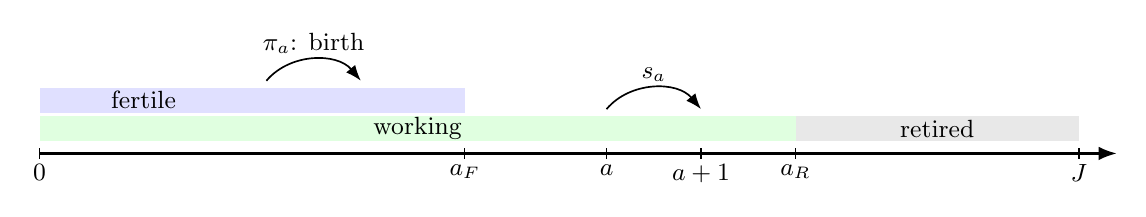
\begin{tikzpicture}[x=1.2cm,y=0.45cm,font=\small]
 \fill[blue!12] (0,0.65) rectangle (4.5,1.35); \node at (1.1,1) {fertile};
 \draw[-Latex,semithick] (2.4,1.55) to[bend left=50] node[above,inner sep=2pt] {$\pi_a$: birth} (3.4,1.55);
 \fill[green!12] (0,-0.15) rectangle (8,0.55); \node at (4,0.2) {working};
 \fill[gray!18] (8,-0.15) rectangle (11,0.55); \node at (9.5,0.2) {retired};
 \draw[thick,-Latex] (0,-0.5) -- (11.4,-0.5);
 \foreach \x/\l in {0/{$0$},4.5/{$a_F$},6/{$a$},7/{$a+1$},8/{$a_R$},11/{$J$}}
  {\draw (\x,-0.65) -- (\x,-0.35); \node[below,inner sep=2pt] at (\x,-0.65) {\l};}
 \draw[-Latex,semithick] (6,0.75) to[bend left=50] node[above,inner sep=2pt] {$s_a$} (7,0.75);
\end{tikzpicture}
\caption{Life cycle of a household. Until age $a_F$, a try for a child
succeeds with probability $\pi_a$, which declines with age. A household of age $a$ survives to age
$a+1$ with probability $s_a$.}
\label{fig:m-lifecycle}
\end{figure}

Households value consumption $c_t$, housing services $\hat h_t$ and the
number of children at home $n_t$, and discount the future by $\beta$. A
household either owns $h^O_t$ or rents $h^R_t$, and its housing services are
\begin{equation*}
 \hat h_t=\begin{cases}\chi\,h^O_t, & \text{owner},\\ h^R_t, & \text{renter},\end{cases}
 \qquad \chi>1 .
\end{equation*}
The parameter $\chi$ determines the additional services a household obtains
from owning a home of a given size. Flow utility is
\begin{equation}
 u(c_t,\hat h_t,n_t)=\frac{1}{1-\sigma}\left[\frac{c_t^{\alpha_0}\bigl(\hat h_t-\chi^{\1\{\text{own}\}}\,\bar h(n_t)\bigr)^{1-\alpha_0}}{e(n_t)}\right]^{1-\sigma}+\psi_t\,v(n_t),
 \label{eq:m-utility}
\end{equation}
with
\begin{equation*}
 \bar h(n_t)=h_P\,\1\{n_t>0\},\qquad v(n_t)=n_t^{1-\gamma}.
\end{equation*}
The first term is utility from a Cobb--Douglas composite of consumption and
housing services above a requirement $\bar h(n_t)$, per adult equivalent,
where $\alpha_0$ is the weight on consumption and $\sigma$ the curvature.
Children raise the household's needs in two ways. First, a household with
children at home must occupy $h_P$ units of housing before additional housing
yields services; an owner obtains $\chi(h^O_t-h_P)$ and a renter $h^R_t-h_P$.
The requirement does not depend on the number of children, so the first
child activates it, and the household pays for it every period its children
are at home, whether it rents or owns. Second, the equivalence scale
$e(n_t)$, with $e(0)=1$, measures adult equivalents relative to a childless
couple.\footnote{I use the scale of
\citet{scholzSeshadriKhitatrakunSaving2006},
$e(n_t)=\bigl((2+\omega n_t)/2\bigr)^{\nu}$, where $\omega$ is the weight of
a child relative to an adult and $\nu$ governs economies of scale.} The second
term, $\psi_t v(n_t)$, is the benefit of children at home: $\psi_t$ is the
preference for children and $\gamma$ governs how fast the benefit of an
additional child declines. The first child also carries a one-time utility
cost $\xi$ at birth. \textcolor{red}{[To recheck: whether the first-birth
cost $\xi$ is needed.]}

\textcolor{red}{[Check: the code applies $\chi$ to the requirement for owners, so owner services above it are $\chi(h^O_t-h_P)$, as written here; the deck's Utility Specification slide writes $\chi h^O_t-h_P$.]}

\subsubsection*{Bequests.}
A household that dies at the end of period $t$ leaves the estate
$x_{t+1}=b_{t+1}+(1-\mu)P_th^O_t$, its bond position and the value of its
home net of the selling cost. As in \citet{deNardiWealthInequality2004}, it
values the estate according to
\begin{equation*}
 B(x_{t+1})=\theta_0\,\frac{(\theta_1+x_{t+1})^{1-\sigma}}{1-\sigma},
\end{equation*}
where $\theta_0$ scales the strength of the bequest motive and $\theta_1$
determines the extent to which bequests are a luxury good. Estates are
collected by the government.

\subsubsection*{Income.}
Before retirement, a household supplies one unit of labor inelastically, with
efficiency $e_az_t$. The term $e_a$ is the age profile of earnings, and $z_t$
is idiosyncratic labor efficiency, whose logarithm follows a first-order
autoregressive process,
\begin{equation*}
 \log z_{t+1}=\rho_z\log z_t+\epsilon_{t+1},\qquad
 \epsilon_{t+1}\sim N(0,\sigma_z^2),
\end{equation*}
where $\rho_z$ is the persistence and $\sigma_z^2$ the variance of the
innovations. Earnings are taxed at rate
$\tau^w$, and retirees receive a pension $m_t$:
\begin{equation*}
 y_t(a,z_t)=\begin{cases}(1-\tau^w)\,w\,e_az_t, & a<a_R,\\ m_t, & a\ge a_R.\end{cases}
\end{equation*}
Every household also receives a transfer $T_t$, the rebate of property-tax
revenue.

\subsubsection*{Housing.}
A household enters period $t$ with the home it owned in the previous period,
$h^O_{t-1}$, which is zero for a renter. Owner-occupied homes come in a finite
set of sizes, $h^O_t\in\mathcal H$, and trade at price $P_t$ per unit of
space. Owners pay maintenance $\delta_H$ and property tax $\tau^p$ on the
value of their home, $P_th^O_t$, and selling a home costs a fraction $\mu$ of
its value. Renters choose any size up to a cap, $h^R_t\le\bar h^R$, at rent
$r_t$ per unit. Since $\bar h^R<\max\mathcal H$, the largest homes are only
for sale.

\subsubsection*{Borrowing.}
Households save or borrow in a one-period bond, traded with the rest of the
world at the exogenous gross return $R_b$. Let $b_{t+1}$ denote the bond
position a household chooses in period $t$.
Borrowing must be secured by a home, so a renter cannot borrow,
$b_{t+1}\ge0$. An owner can borrow up to a fraction $\phi$ of the current
value of its home:
\begin{equation}
 b_{t+1}\ge-\phi\,P_th^O_t .
 \label{eq:m-ltv}
\end{equation}
The limit applies both to a household that buys a home and to one that stays
in the home it owns. A buyer must therefore pay at least $(1-\phi)P_th^O_t$
itself, out of its bond position, the income of the period and the proceeds
from selling any home it owned. This down payment ties ownership, and with it
access to the largest homes, to the household's wealth. Debt is rolled over
each period at the return $R_b$: mortgages have no amortization schedule and
no limit on payments relative to income.

\subsubsection*{Fertility.}
Until age $a_F$, a household decides each period whether to try to have a
child. A try succeeds with probability $\pi_a$, which declines with age, and a
success adds one child at home in the same period. Children do not work and
make no decisions; they affect the household through its needs and through
the benefit of children in preferences. Each child at home leaves with
probability $\lambda$ per period, independently of its siblings, so a child
stays at home for $1/\lambda$ periods on average. Children who leave form new
households and enter the economy at age $0$, with an initial wealth position
drawn from an exogenous distribution.

\subsubsection*{Housing supply.}
Housing is built by absentee developers, who sell it to households and to
landlords at the price $P_t$ per unit. I do not model the construction
technology explicitly. Instead, the aggregate housing stock is an increasing
function of the current price,
\begin{equation}
 H_t=H_0\,P_t^{\eta},
 \label{eq:m-supply}
\end{equation}
where $H_0>0$ sets the scale of the stock and $\eta\ge0$ is the price
elasticity of housing supply. The stock in period $t$ depends only on the
price in period $t$, so supply adjusts within the period. The elasticity
governs how a change in the demand for housing is split between the price and
the quantity. When $\eta=0$ the stock is fixed and the price absorbs the whole
change; the larger is $\eta$, the more the stock adjusts and the less the
price moves. The stock is divided between owner-occupied and rental housing
by households' tenure choices.

\subsubsection*{Rental market.}
A household that does not own a home rents from landlords. Landlords are
competitive and owned by agents outside the economy. A landlord buys housing
at the price $P_t$, rents it to households at the rent $r_t$ per unit, pays
maintenance and property tax on its value, $(\delta_H+\tau^p)P_t$, and sells
it at the price $P_{t+1}$ in the next period. Landlords finance their
purchases at the gross return $R_b$ and, unlike households, pay no
transaction cost when they sell. Competition drives their profit to zero, so
the return on a unit of rental housing equals the return on the bond:
\begin{equation}
 r_t+P_{t+1}-(\delta_H+\tau^p)P_t=R_b\,P_t .
 \label{eq:m-rent}
\end{equation}
Landlords supply any quantity of rental housing at this rent. Rearranging,
\begin{equation*}
 r_t=(R_b-1+\delta_H+\tau^p)\,P_t-(P_{t+1}-P_t).
\end{equation*}
The rent equals the user cost of housing: the interest forgone on the price,
plus maintenance and property tax, net of the capital gain. The rent
therefore depends on the expected path of the price, not only on its current
level. When the price is expected to fall, the rent rises relative to the
price, because landlords must be compensated for the expected capital loss. \textcolor{red}{[To review: written as on the slides and in the production
code. How maintenance and the rent are accounted for, for owners and for
landlords, is under review (accounting test, Oct 17).]}

\subsubsection*{Firms.}
A representative firm produces the consumption good, which is the numeraire,
with a linear technology in effective labor,
\begin{equation*}
 Y_t=A\,L_t,\qquad L_t=\int_{a<a_R}e_az_t\,\dd G_t,
\end{equation*}
where $A$ is productivity, $G_t$ is the measure of households over states and
$L_t$ is the total efficiency units of labor supplied by households of working
age. The firm is competitive and pays each efficiency unit its marginal
product, $w=A$. The wage is therefore constant over time.

\subsubsection*{Government.}
The government runs a pay-as-you-go pension system, taxes housing and collects
estates. It taxes
earnings at the constant rate $\tau^w$ and pays the same pension $m_t$ to
every retired household. The pension system balances its budget every period,
so the pension equals payroll-tax revenue divided by the number of retired
households. When the number of retirees rises relative to effective labor, the
pension falls. The government also levies the property tax $\tau^p$ on the
value of all housing, owned and rented, and returns the revenue to households
as a lump-sum transfer $T_t$, equal across households. Finally, the government
collects the estates of the households that die. It uses them to pay new
households their initial wealth and spends the remainder on government
consumption, which does not affect households.

\subsection{The household's problem}
\label{sec:m-household}

I next characterize the household's problem recursively. A period has two
stages, shown in Figure~\ref{fig:m-timing}. At the beginning of the period,
the household observes its fertility taste shocks and decides whether to try
for a child. After the birth outcome, it observes its housing taste shocks and
chooses its home and saving. A birth therefore changes the demand for housing
in the same period. The state of a household is its bond position $b_t$, the
home it owns $h^O_{t-1}$, its efficiency $z_t$, its age $a_t$ and the number of
children at home $n_t$.

\begin{figure}[ht]
\centering
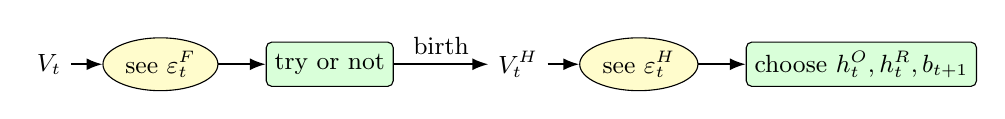
\begin{tikzpicture}[node distance=5mm and 6mm, >=Latex, font=\small,
 see/.style={ellipse, draw, fill=yellow!20, minimum height=1.4em, inner sep=2pt, align=center},
 choose/.style={rectangle, draw, fill=green!15, rounded corners=2pt, minimum height=1.6em, inner sep=3pt, align=center},
 line/.style={-Latex, semithick}]
\node (vt) {$V_t$};
\node (fertS) [see, right=4mm of vt] {see $\varepsilon^F_t$};
\node (fertD) [choose, right=of fertS] {try or not};
\node (vh) [right=12mm of fertD] {$V^H_t$};
\node (locS) [see, right=4mm of vh] {see $\varepsilon^H_t$};
\node (locD) [choose, right=of locS] {choose $h^O_t,h^R_t,b_{t+1}$};
\draw[line] (vt) -- (fertS);
\draw[line] (fertS) -- (fertD);
\draw[line] (fertD) -- node[above]{birth} (vh);
\draw[line] (vh) -- (locS);
\draw[line] (locS) -- (locD);
\end{tikzpicture}
\caption{Timing within period $t$.}
\label{fig:m-timing}
\end{figure}

\subsubsection*{Fertility.}
Let $V_t(b_t,h^O_{t-1},z_t,a_t,n_t)$ denote the value of a household at the
beginning of period $t$, before it observes its fertility shocks. A household
of fertile age chooses between not trying, $j=0$, and trying, $j=A$. Each
option receives a taste shock
$\varepsilon^F_{t,j}\overset{iid}{\sim}\text{Gumbel}(0,\kappa)$, with
$\kappa=\kappa_1$ before the first child and $\kappa=\kappa_C$ after. The
separate scales allow the decision to become a parent to respond differently
from the decision to have another child. The value of the household and the
probability of trying are
\begin{equation}
\begin{aligned}
 V_t&=\E_{\varepsilon^F_{t,j}}\max_{j\in\{0,A\}}\bigl\{V^F_{t,j}+\varepsilon^F_{t,j}\bigr\}
 =\kappa\log\bigl[\exp\bigl(V^F_{t,0}/\kappa\bigr)+\exp\bigl(V^F_{t,A}/\kappa\bigr)\bigr],\\
 \pi^F_{t,a}&=\frac{\exp\bigl(V^F_{t,A}/\kappa\bigr)}{\exp\bigl(V^F_{t,0}/\kappa\bigr)+\exp\bigl(V^F_{t,A}/\kappa\bigr)},
\end{aligned}
 \label{eq:m-fertility}
\end{equation}
where $V^F_{t,0}$ and $V^F_{t,A}$ are the values of not trying and trying
before the shocks. Both depend on $V^H_t$, the value of the household after the
birth outcome, which I define below:
\begin{equation*}
\begin{aligned}
 V^F_{t,0}&=V^H_t(b_t,h^O_{t-1},z_t,a_t,n_t),\\
 V^F_{t,A}&=\pi_a\bigl[V^H_t(b_t,h^O_{t-1},z_t,a_t,n_t+1)-\xi\,\1\{\text{first child}\}\bigr]+(1-\pi_a)\,V^F_{t,0}.
\end{aligned}
\end{equation*}
Not trying leaves the number of children at home unchanged. Trying succeeds
with probability $\pi_a$, adds a child at home and, for the first child,
carries the utility cost $\xi$; if it fails, the household is in the same
position as if it had not tried. Given its state, a household has a child
with probability $\pi_a\pi^F_{t,a}$. Outside the fertile ages, there is no
fertility choice and $V_t=V^H_t(b_t,h^O_{t-1},z_t,a_t,n_t)$.

\subsubsection*{Housing and savings.}
After the birth outcome, the household observes its housing taste shocks and
chooses its home, its tenure and its bond position. Let $n_{t+1}$ denote the
number of children at home after this period's birth outcome. Before the
housing shocks, the value of the household is
\begin{multline}
 V^H_t(b_t,h^O_{t-1},z_t,a_t,n_{t+1})
 =\E_{\varepsilon^H_{t,j}}\max_{h^O_t,h^R_t,b_{t+1}}
 \Bigl\{u(c_t,\hat h_t,n_{t+1})+\varepsilon^H_{t,j}\\
 +\beta\,\E_t\Bigl[s_aV_{t+1}(b_{t+1},h^O_t,z_{t+1},a_t+1,n_{t+1})
 +(1-s_a)B(x_{t+1})\Bigr]\Bigr\},
 \label{eq:m-vh}
\end{multline}
subject to the budget constraint of the chosen option,
\begin{equation}
\begin{aligned}
 &\text{Buy:}  && c_t+b_{t+1}+(\delta_H+\tau^p)P_th^O_t=R_bb_t+y_t+T_t-P_t\bigl[h^O_t-(1-\mu)h^O_{t-1}\bigr],\\
 &\text{Stay:} && c_t+b_{t+1}+(\delta_H+\tau^p)P_th^O_t=R_bb_t+y_t+T_t,\\
 &\text{Rent:} && c_t+b_{t+1}+r_th^R_t=R_bb_t+y_t+T_t+(1-\mu)P_th^O_{t-1},
\end{aligned}
 \label{eq:m-budget}
\end{equation}
and the borrowing limit \eqref{eq:m-ltv} for buyers and stayers, or
$b_{t+1}\ge0$ for renters. A buyer sells the home it owns, if any, and buys a
new one; a stayer keeps its home; a renter sells the home it owns, if any, and
rents. The expectation $\E_t$ is over next period's efficiency and the
departure of children. The shocks
$\varepsilon^H_{t,j}\overset{iid}{\sim}\text{Gumbel}(0,\kappa_T)$ are one per
option $j$: renting, or owning each $h^O\in\mathcal H$. Let $V^j_t$ denote the
value of option $j$ before the shock. Then
\begin{equation}
 V^H_t=\kappa_T\log\sum_{j}\exp\bigl(V^j_t/\kappa_T\bigr),
 \qquad
 \pi^H_t(j)=\frac{\exp(V^j_t/\kappa_T)}{\sum_{j'}\exp(V^{j'}_t/\kappa_T)},
 \label{eq:m-tenure}
\end{equation}
where $\pi^H_t(j)$ is the probability of choosing option $j$. \textcolor{red}{[To consider: dropping the
tenure taste shocks $\varepsilon^H_{t,j}$.]} An option that
leaves no saving choice within the budget and borrowing constraints cannot be
chosen. Housing costs, credit and earnings risk shape $V^H_t$, and through it
the gap $V^F_{t,A}-V^F_{t,0}$ that governs fertility.

\subsection{Equilibrium}
\label{sec:m-equilibrium}

\textcolor{red}{[To review: the equilibrium definition.]}

\begin{definition}
Given an initial measure of households over states $G_0$, an equilibrium is
a path of prices $\{P_t,r_t\}$, pensions $\{m_t\}$, rebates $\{T_t\}$, value
and policy functions, and measures $\{G_t\}$ consistent with the policy
functions, the shocks, survival and entry, such that every period:
\begin{enumerate}
\item \emph{Households} solve their problem, given prices, transfers and
shocks, and rent satisfies the landlords' zero-profit condition
\eqref{eq:m-rent}.
\item \emph{Housing market} clears: owned and rented housing equal the stock,
\[
 \int\bigl(h^O_t+h^R_t\bigr)\,\dd G_t=H_t .
\]
\item \emph{Pensions}: payroll taxes pay the pensions of the $N^R_t$ retired
households, $\tau^wwL_t=m_tN^R_t$.
\item \emph{Rebate}: property-tax revenue is paid to all $N_t$ households,
$T_tN_t=\tau^pP_t\int\bigl(h^O_t+h^R_t\bigr)\,\dd G_t$.
\item \emph{Population}: births are $B_t=\int\pi_a\pi^F_{t,a}\,\dd G_t$, and
new households are $E_t=\lambda K_t$, where $K_t$ is the number of children
at home.
\end{enumerate}
\end{definition}

\begin{definition}
A stationary equilibrium is a price $P$, a rent $r$, a pension $m$, a rebate
$T$, value and policy functions, and a measure of households over states
$G$, such that:
\begin{enumerate}
\item \emph{Households} solve their problem, given $P$, $r$, $m$ and $T$.
\item \emph{Rent} satisfies the landlords' zero-profit condition at a
constant price, $r=(R_b-1+\delta_H+\tau^p)P$.
\item \emph{Housing market} clears,
$\int\bigl(h^O+h^R\bigr)\,\dd G=H_0P^{\eta}$.
\item \emph{Pensions and rebate} balance, $\tau^wwL=mN^R$ and
$TN=\tau^pP\int\bigl(h^O+h^R\bigr)\,\dd G$.
\item \emph{The measure $G$ is invariant}: the policy functions, the shocks,
survival and the entry of $E=\lambda K$ new households map $G$ into itself.
\end{enumerate}
\end{definition}

\subsection{Model analysis}
\label{sec:m-analysis}

Three tensions shape fertility in the model. The first is timing: the chance
of a birth falls with age, while earnings and wealth rise, and owning the
space a child needs takes a down payment. The second is risk: the child's
space is paid for in every period the child is at home, out of uncertain
earnings. The third runs through the housing market: fewer children lower the
demand for housing and its price, and a lower price raises fertility.
Section~\ref{sec:results} measures the cost of the child's space and the role
of risk, Section~\ref{sec:policy-credit} the role of the down payment, and
Section~\ref{sec:quant-transition} the response of the housing market.

\subsubsection*{Borrowing limits and the timing of children.}
A try for a child succeeds with probability $\pi_a$, which declines with age,
while earnings $e_az_t$ rise with age through $e_a$
(Figure~\ref{fig:m-agetiming}a). A child raises by $r_th_P$ the spending
needed for the same housing services, in every period it is at home. The home
a family wants also requires a down payment: a renter cannot borrow, and an
owner can borrow only against its home. Let $\zeta_t\ge0$ denote the
multiplier on the borrowing limit, $b_{t+1}\ge-\phi P_th^O_t$ with $h^O_t=0$
for a renter: the value, in utility, of borrowing one more unit in period
$t$.\footnote{Appendix~\ref{app:household} derives the Euler equation for the
bond and the conditions behind the results below.} A birth raises the
multiplier when it raises marginal utility more today than next period, as
for a household whose earnings rise. Such a household can delay the child, at
the cost of a lower $\pi_a$. It can have the child in rented space and forgo
$\chi$ and the homes larger than $\bar h^R$. Or it can have the child and buy
once its savings cover the down payment.

\begin{figure}[ht]
\centering
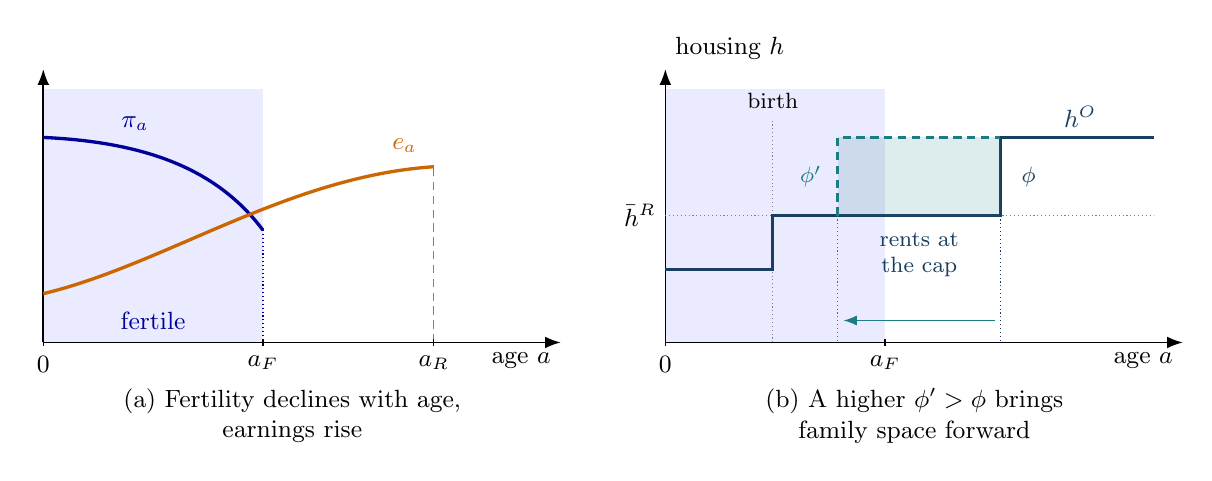
\begin{tikzpicture}[>=Latex,font=\small]
\begin{scope}[x=0.62cm,y=0.62cm]
 \fill[blue!8] (0,0) rectangle (4.5,5.2);
 \node[text=blue!60!black] at (2.25,0.45) {fertile};
 \draw[->,semithick] (0,0) -- (10.6,0) node[below left] {age $a$};
 \draw[->,semithick] (0,0) -- (0,5.6);
 \draw[very thick,blue!60!black] (0,4.2) .. controls (2.2,4.1) and (3.6,3.5) .. (4.5,2.3);
 \draw[blue!60!black,densely dotted] (4.5,2.3) -- (4.5,0);
 \node[text=blue!60!black,anchor=south west] at (1.4,4.15) {$\pi_a$};
 \draw[very thick,orange!80!black] (0,1.0) .. controls (2.5,1.6) and (5,3.4) .. (8,3.6);
 \node[text=orange!80!black,anchor=south] at (7.4,3.7) {$e_a$};
 \draw[densely dashed,gray] (8,0) -- (8,3.6);
 \foreach \x/\l in {0/{$0$},4.5/{$a_F$},8/{$a_R$}}
  {\draw (\x,0.08) -- (\x,-0.08); \node[below] at (\x,-0.08) {\l};}
 \node[align=center] at (5.1,-1.5) {(a) Fertility declines with age,\\ earnings rise};
\end{scope}
\begin{scope}[xshift=7.9cm,x=0.62cm,y=0.62cm]
 \fill[blue!8] (0,0) rectangle (4.5,5.2);
 \draw[->,semithick] (0,0) -- (10.6,0) node[below left] {age $a$};
 \draw[->,semithick] (0,0) -- (0,5.6) node[above right] {housing $h$};
 \draw[densely dotted,gray] (0,2.6) -- (10,2.6); \node[left] at (0,2.6) {$\bar h^R$};
 \draw[densely dotted,gray] (2.2,0) -- (2.2,4.6); \node[anchor=south,font=\footnotesize] at (2.2,4.6) {birth};
 \draw[very thick,mechnavy] (0,1.5) -- (2.2,1.5) -- (2.2,2.6) -- (3.53,2.6);
 \draw[very thick,mechnavy] (3.53,2.6) -- (6.86,2.6) -- (6.86,4.2) -- (10,4.2);
 \draw[very thick,mechteal,densely dashed] (3.53,2.6) -- (3.53,4.2) -- (6.86,4.2);
 \fill[mechteal,opacity=0.15] (3.53,2.6) rectangle (6.86,4.2);
 \node[text=mechnavy,anchor=south] at (8.5,4.2) {$h^O$};
 \node[text=mechnavy,anchor=north,font=\footnotesize,align=center] at (5.2,2.45) {rents at\\ the cap};
 \draw[->,mechteal] (6.75,0.45) -- (3.65,0.45);
 \draw[mechnavy,densely dotted] (6.86,2.6) -- (6.86,0);
 \draw[mechteal,densely dotted] (3.53,2.6) -- (3.53,0);
 \foreach \x/\l in {0/{$0$},4.5/{$a_F$}}
  {\draw (\x,0.08) -- (\x,-0.08); \node[below] at (\x,-0.08) {\l};}
 \node[text=mechnavy,anchor=west,font=\footnotesize] at (7.1,3.4) {$\phi$};
 \node[text=mechteal,anchor=east,font=\footnotesize] at (3.4,3.4) {$\phi'$};
 \node[align=center] at (5.1,-1.5) {(b) A higher $\phi'>\phi$ brings\\ family space forward};
\end{scope}
\end{tikzpicture}
\caption{Timing of fertility, earnings and the purchase of a family home}
\label{fig:m-agetiming}
\par\smallskip
\begin{minipage}{0.92\linewidth}
\footnotesize\textit{Notes:} Schematic. The shaded area marks the fertile
ages. In panel (b), the solid line is the housing of a household that rents
until its savings cover the down payment on a family home $h^O$ at the
loan-to-value ratio $\phi$. The dashed line is the same household at
$\phi'>\phi$, and the shaded area is the family space it gains.
\end{minipage}
\end{figure}

A higher loan-to-value ratio $\phi$ lowers the equity $(1-\phi)P_th^O_t$ a
buyer needs and allows an earlier purchase (Figure~\ref{fig:m-agetiming}b).
It leaves the cost of a child's space unchanged: by \eqref{eq:m-rent}, that
space costs about $r_th_P$ every period, whether the household rents or
owns.\footnote{Apart from the selling cost, an owner that holds a unit from
$t$ to $t+1$ pays $(1+\tau^p)P_t$ in period $t$ and holds $(1-\delta_H)P_{t+1}$
in period $t+1$, so by \eqref{eq:m-rent} its cost, in period-$t$ units, equals
the rent $r_t$.} For a change in $\phi$ in period $t$, the envelope theorem,
\eqref{eq:m-tenure} and \eqref{eq:m-fertility} give\footnote{Here
$\kappa=\kappa_1$ before the first child and $\kappa_C$ after. A permanent
change in $\phi$ adds the corresponding terms for all future periods,
discounted and weighted by survival.}
\begin{equation}
 \begin{gathered}
 \frac{\partial\pi^F_{t,a}}{\partial\phi}
 =\frac{\pi^F_{t,a}\bigl(1-\pi^F_{t,a}\bigr)}{\kappa}\;\pi_a
 \left[\frac{\partial V^H_t(n_t+1)}{\partial\phi}-\frac{\partial V^H_t(n_t)}{\partial\phi}\right],
 \\
 \frac{\partial V^H_t(n)}{\partial\phi}
 =\sum_{h^O\in\mathcal H}\pi^H_t(h^O\mid n)\,\zeta_t(h^O,n)\,P_th^O ,
 \end{gathered}
 \label{eq:m-credit}
\end{equation}
where $\pi^H_t(h^O\mid n)$ is the probability of owning $h^O$ and
$\zeta_t(h^O,n)$ the multiplier in that option. The second line is the value
of credit to a household with $n$ children at home: an owner of $h^O$ can
borrow $P_th^O$ more, and each unit is worth $\zeta_t(h^O,n)$. Credit is worth
nothing to a household that rents or whose limit is slack. The first line
says that credit raises the probability of trying only through the difference
between its value with the additional child and without it. The difference is
positive when the child moves the household toward larger owned homes, where
the limit binds, close to zero for a household that rents either way, and
negative when credit mainly helps households without children to buy. The
factor in front is largest for households close to indifferent about trying
and falls with age through $\pi_a$. Section~\ref{sec:policy-credit} shows
which case dominates in the calibrated model: credit mostly lets young
households buy the small homes they would otherwise rent, and it brings
births forward.

\subsubsection*{Earnings risk.}
A child stays at home for $1/\lambda$ periods on average, while earnings are
risky and persistent. Consider a renter at the borrowing limit,
$b_t=b_{t+1}=0$, that rents below the cap. Maximizing \eqref{eq:m-utility}
subject to $c_t+r_th^R_t=y_t+T_t$ gives the flow utility
\begin{equation}
 u(c_t,h^R_t,n_t)=\frac{1}{1-\sigma}\left[\frac{\alpha_0^{\alpha_0}(1-\alpha_0)^{1-\alpha_0}}{r_t^{1-\alpha_0}}\;
 \frac{y_t+T_t-r_t\bar h(n_t)}{e(n_t)}\right]^{1-\sigma}+\psi_t\,v(n_t).
 \label{eq:m-indirect}
\end{equation}
The child's space is a committed expenditure, paid out of income before the
household divides the rest between consumption and additional space. Let
$\Delta_t(y_t)$ be the utility cost of a first child: the first term of
\eqref{eq:m-indirect} with $n_t=0$ minus the same term with $n_t=1$. For
$\sigma\ge1$, $\Delta_t$ is decreasing and convex in earnings, and more convex
when $r_th_P$ is larger.\footnote{Let $\tilde y_t=y_t+T_t$, $k=r_th_P$ and
$\Theta_t=\alpha_0^{\alpha_0}(1-\alpha_0)^{1-\alpha_0}r_t^{\alpha_0-1}$. Then
$\Delta_t''(\tilde y_t)=\sigma\Theta_t^{1-\sigma}\bigl[e(1)^{\sigma-1}(\tilde y_t-k)^{-\sigma-1}-\tilde y_t^{-\sigma-1}\bigr]$,
which is positive for $\sigma\ge1$, since $e(1)\ge1$ and $k>0$, and rises
with $k$.} By Jensen's inequality, earnings risk raises the expected cost of a
child above its cost at expected earnings, and by more when the child's space
is more expensive (Figure~\ref{fig:m-risk}). Savings soften this effect.
Section~\ref{sec:results-risk} measures it in the calibrated model.

\begin{figure}[ht]
\centering
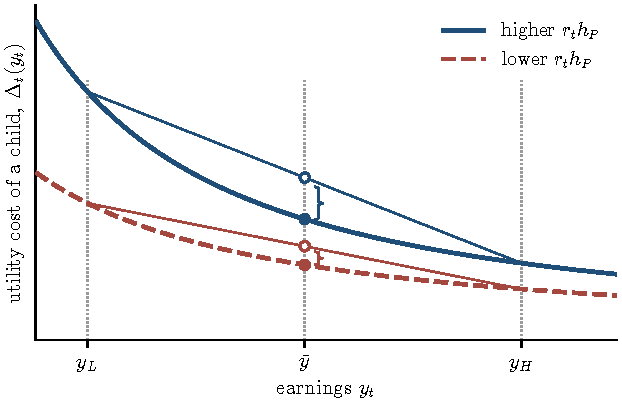
\includegraphics[width=0.65\textwidth]{figures/fig_m_risk_fi.pdf}
\caption{Earnings risk and the utility cost of a child}
\label{fig:m-risk}
\par\smallskip
\begin{minipage}{0.92\linewidth}
\footnotesize\textit{Notes:} The figure is computed from \eqref{eq:m-indirect} at the
parameters of Section~\ref{sec:quant} (Appendix~\ref{app:model-figures}).
The curves plot $\Delta_t$ for a renter at the borrowing limit, at the rent of
the initial steady state (solid) and at the rent of the new steady state of
Figure~\ref{fig:m-illustration} (dashed). Earnings are $y_L$ or $y_H$ with
equal probability. Filled circles mark the cost at expected earnings $\bar y$
and open circles the expected cost; the braces mark the additional cost due to
risk.
\end{minipage}
\end{figure}

\subsubsection*{Households and the housing market.}
Figure~\ref{fig:m-illustration} shows how the economy responds to a fall in
the preference for children, from $\psi_0$ to $\psi_1$. Panel (a) shows the
housing market in a steady state. Supply \eqref{eq:m-supply} rises with the
price. Demand, $N\,h(P;\psi)$, is the number of households $N$ times the
housing each one owns or rents at the price $P$.\footnote{In a steady state,
the housing market (Section~\ref{sec:m-equilibrium}) clears when this demand equals the stock.
Housing and fertility respond to the rent. In a steady state, the rent is
proportional to the price by \eqref{eq:m-rent}, so both can be read against
the price. Along a transition, the rent also reflects the expected change in
the price.} Panel (b) shows the fertility $n(P;\psi)$ that households choose
at each price. At $A$, the market clears at $P_0$ with $N_0$ households, and
fertility is at the replacement rate $\bar n$. When the preference falls, the
population is inherited and the price stays close to $P_0$, so fertility
falls along $n(P;\psi_1)$, from $A$ to $A'$. Over the following generations,
smaller cohorts reduce the number of households, demand shifts left, and the
price falls along the supply curve. The lower price raises fertility along
$n(P;\psi_1)$, until fertility is back at replacement at $B$, with fewer
households and cheaper housing. The transition of
Section~\ref{sec:quant-transition} follows these steps.

In a steady state, the number of new households equals the number that die,
so fertility is at the replacement rate. Since the household problem, the
pension and the rebate per household do not depend on the number of
households, the condition $n(P;\psi)=\bar n$ in panel (b) determines the
steady-state price, and supply and demand in panel (a) then determine the
number of households. A more elastic supply therefore leaves the steady-state
price unchanged and implies a larger fall in the number of households.

\begin{figure}[ht]
\centering
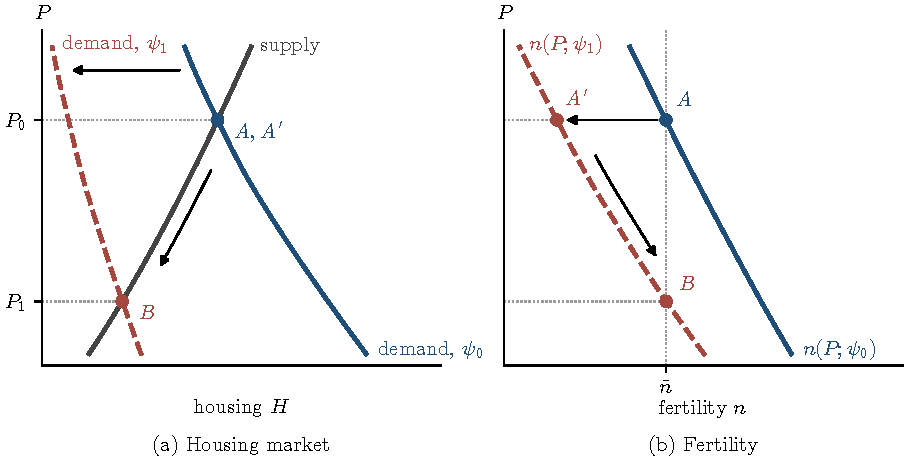
\includegraphics[width=\textwidth]{figures/fig_m_illustration_demand.pdf}
\caption{The housing market and fertility}
\label{fig:m-illustration}
\par\smallskip
\begin{minipage}{0.92\linewidth}
\footnotesize\textit{Notes:} The figure is computed from stationary solves of
the model at given prices, at the parameters of Section~\ref{sec:quant}
(Appendix~\ref{app:model-figures}). Panel (a) shows housing supply
\eqref{eq:m-supply} and demand with $N_0$ households under $\psi_0$ (solid)
and $N_1$ households under $\psi_1$ (dashed). Panel (b) shows the fertility
households choose at each price; the dotted line marks replacement. $A$ is the
initial steady state, $A'$ the outcome at the inherited population after the
fall in $\psi$, and $B$ the new steady state.
\end{minipage}
\end{figure}

% Shipped from the mock (latex/JMP_DS_mock/sections/04_quantification.tex) on Oct 26 2026, his word (fecundity and e_a sentences).
% Section 4 at the recalibrated new-accounting point (loss 7.4186), Oct 21 2026.
% Parameters and 2007 fit: output/model/calibration/2026-10-19_identification_newacct/
% (torch/best_point.json; moments/center.json: target_fit, event paths, price, loss).
% Mothers by 25 and 2007 life-cycle: output/model/calibration/2026-10-21_lifecycle_newacct/
% (Results write-up thread's fixed-price 2007 solve).
% Transition (Oct 24, free entry main): FIN063fi_fw.json (eta 0.63, free entry, rho 0.35, psi_inf
% 0.148414), in output/model/experiments/housing_supply/20261022_fi_all_arms/history/.
% 2023 table and life-cycle: .../housing_supply/20261021_free_entry/moments_2023_fi/ (free_entry_eta0.63
% column; same observers as the 7.9 table, replay of the converged FIN063fi_fw history).
% Oct 25: 4.1-4.2 restructured on the model of Boar, Gorea and Midrigan (2017, Sec. 4.1, Table 2);
% Section 5 (Testing the model) is in 05_testing.tex.

\section{Quantification}
\label{sec:quant}
\label{sec:quantification}

In this section, I describe the quantification of the model. Because
fertility rates vary a lot over time and the age distribution of the
population reflects many years of past fertility decisions, some assumptions
are needed to make the quantification tractable. To this end, I approximate
the United States economy of 2007 with a steady state in which births are at
replacement. I parameterize the model so that this steady state matches
fertility, housing and wealth moments of 2007. Holding these parameters
fixed, I then let the preference for children $\psi_t$ fall after 2007 so
that the model matches the decline in fertility until 2023, and I solve for
the transition of the economy as prices, family composition and household
entry adjust (Section~\ref{sec:quant-transition}). I treat this fall as an
exogenous shock to preferences and take it as given. The 2023 state of this
transition is the starting point of the policy experiments in
Section~\ref{sec:policy}.

\subsection{Quantification strategy}
\label{sec:quant-approach}

Two measures of fertility guide the quantification
(Figure~\ref{fig:quant-us-fertility}). Period fertility, or the total
fertility rate, is the number of children a woman would have if she lived
through her fertile years at the birth rates of a given year. Completed
fertility is the number of children a woman has had by the end of her fertile
years. I measure it at ages 40 to 44. Whether a population replaces itself
depends on completed fertility, which is then the key number to look at when thinking about population growth trends. In a steady state the two measures coincide. Out of
a steady state, completed fertility lags period fertility, because it adds up
the births of a cohort over two decades. In the United States, period
fertility peaked at about 2.1 in 2007 and fell to 1.62 by 2023, while
completed fertility was still 1.92 in 2024. If period fertility stayed at its
2023 level, completed fertility would fall to 1.62 within about two decades,
as the cohorts that had their children before 2007 age out.\footnote{The
same lag explains why the number of households does not fall at once when
fertility falls: fewer births lower the number of new households only when
the smaller cohorts reach adulthood. This is also why, despite almost two
decades of below-replacement period fertility, the population of the United
States has not yet started to decrease.}
% Model: households 1.000 through the period dated 2019, 0.997 in 2023, 0.989 in 2027
% (FIN063fi_fw.json rows adult_population).

\begin{figure}[!htbp]
\centering
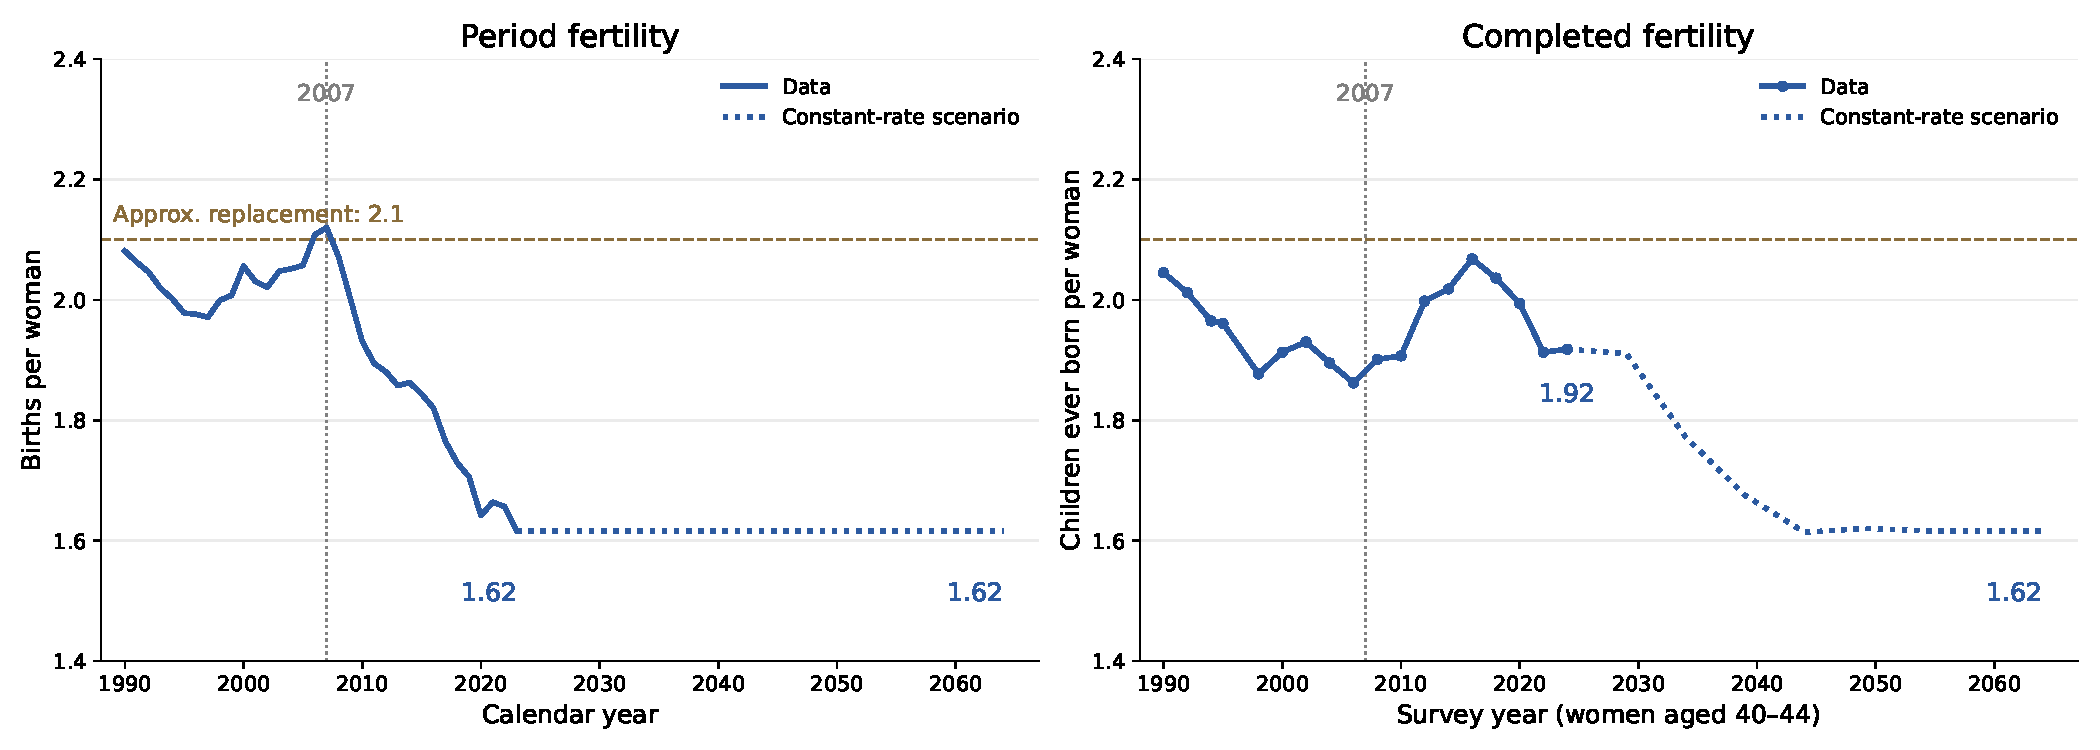
\includegraphics[width=\linewidth]{fertility_introduction_projection_1990}
\caption{Period and completed fertility in the United States}
\label{fig:quant-us-fertility}
\par\smallskip
\begin{minipage}{0.92\linewidth}
\footnotesize\textit{Notes:} Left: period total fertility rate, World
Development Indicators. Right: children ever born to women aged 40--44, CPS
Fertility Supplement. Dotted lines: a constant-rate scenario that holds period
fertility at its 2023 level; the completed-fertility continuation is rescaled
to end at that rate.
\end{minipage}
\end{figure}

The transition follows the logic of Section~\ref{sec:m-analysis}: fertility
falls first at about the inherited price, and the price falls as smaller
cohorts enter. I compare each policy experiment with the path the economy
follows from 2023 without it.

I divide the parameters of the 2007 economy into two groups. The first
group is assigned from external evidence or measured directly in the data.
The second is chosen so that the model matches a set of moments in the data.
Table~\ref{tab:quant-moments} reports the moments, and
Table~\ref{tab:quant-parameters} the parameters.

\subsection{Assigned parameters}
\label{sec:quant-data}
\label{sec:quant-period}

\begin{table}[!htbp]
\centering
\caption{Parameter values}
\label{tab:quant-parameters}
\small
\begin{tabularx}{\textwidth}{@{}l l X @{\hspace{1.5em}} l l X@{}}
\toprule
\multicolumn{3}{@{}l}{Assigned} & \multicolumn{3}{l}{Calibrated}\\
\midrule
$\sigma$ & 2 & risk aversion & $\beta_{\text{ann}}$ & 0.936 & annual discount factor \\
$(\omega,\nu)$ & 0.7, 0.7 & equivalence scale & $\psi_0$ & 0.177 & preference for children \\
$\alpha_0$ & 0.733 & consumption weight & $\gamma$ & 0.646 & curvature, benefit of children \\
$\lambda$ & $2/9$ & child departure, per period & $\xi$ & 0.295 & first-birth utility cost \\
$\pi_a$ & 0.98--0.50 & success of a birth attempt & $\kappa_1$ & 0.050 & first-birth taste scale \\
$\phi$ & 0.80 & financed share & $\kappa_C$ & 0.129 & later-birth taste scale \\
$\mu$ & 0.06 & selling cost & $h_P$ & 0.89 & space requirement (rooms) \\
$\delta_H$ & 0.014 & depreciation, annual & $\chi$ & 1.112 & owner service multiplier \\
$\tau^p$ & 0.0106 & property tax, annual & $\kappa_T$ & 0.013 & tenure taste scale \\
$r$ & 0.02 & real interest rate, annual & $\theta_0$ & 0.244 & bequest-motive scale \\
$\tau^w$ & 0.08 & payroll tax & $H_0$ & 6.776 & housing supply scale \\
% H0 = 5.7505 / 0.77069^0.63 = 6.776 with eta 0.63; 5.7505 = 2007 housing per household.
$\eta$ & 0.63 & housing-supply elasticity & & & \\
$\bar h^R$ & 6 & rental size cap (rooms) & & & \\
$\theta_1$ & 0.008 & bequest shifter & & & \\
$(\rho_z,\sigma_z)$ & 0.735, 0.484 & earnings, per four years & & & \\
\bottomrule
\end{tabularx}
\par\smallskip
\begin{minipage}{0.95\linewidth}
\footnotesize\textit{Notes:} Assigned parameters are set outside the
calibration (Section~\ref{sec:quant-data}); calibrated parameters are chosen
to match the moments of Table~\ref{tab:quant-moments}
(Section~\ref{sec:quant-identification}).
\end{minipage}
\end{table}

\paragraph{Demographics and timing.}
A period in the model lasts four years. Households enter at 18, retire at 66
and live at most through 85. Survival is certain before retirement and,
after it, follows the 2023 period life table of the Social Security
Administration. Births are possible through age 45. The probability that
an attempt succeeds within a period falls with age as
$\pi_a=1-0.02\,e^{0.134(a-18)}$, and is zero from age 45, using the
exponential form of \citet{sommerFertilityChoiceLife2016}. The schedule gives
0.90 at 30, 0.80 at 35 and 0.62 at 40, close to the probabilities of a
conception leading to a live birth within four years computed by
\citet{leridon2004}, 0.91, 0.84 and 0.64.
% POST-DEADLINE: (1) check that Leridon's four-year success probability is the right object for a model
% attempt (the model has no memory of failed attempts; success depends on age only); (2) run the current
% schedule against the July least-squares fit to Leridon (0.01331, 0.14960), holding all else fixed.
% Leridon numbers checked in the abstract by ChatGPT (Oct 25), not read in full here.
A child leaves home with probability $\lambda=2/9$ per
period, so children stay at home for 18 years on average.%
% pi_a = 1 - 0.02 exp(0.134 (a - 18)); 0.50 at 42. Leridon (2004) four-year
% conception 0.91 / 0.84 / 0.64 at 30 / 35 / 40 (docs/model/e5_target_review_20260724.md).
% Survival: 2023 SSA period life table, four-year ratios
% (docs/model/quantification_note_reaudit_and_study_guide_20260720.md).
\footnote{Stocks, such as wealth and house prices, are in annual units, and
flows, such as income, consumption and rent, accrue over the four years.
Interest, discounting and depreciation compound over the period, so
$R_b=1.02^4$ and $\beta=\beta_{\text{ann}}^4$, and the property tax is four
times its annual rate. A data statistic for an age window weights each
four-year model cell by the share of the cell inside the window.}

\paragraph{Preferences.}
Flow utility \eqref{eq:m-utility} is
\begin{equation*}
 u(c,\hat h,n)=\frac{1}{1-\sigma}\left[\frac{c^{\alpha_0}\bigl(\hat h-\chi^{\1\{\text{own}\}}\,\bar h(n)\bigr)^{1-\alpha_0}}{e(n)}\right]^{1-\sigma}+\psi\,n^{1-\gamma},
 \qquad e(n)=\left(\frac{2+\omega n}{2}\right)^{\nu}.
\end{equation*}
I set the curvature to $\sigma=2$, a common choice in the literature. The equivalence scale
$e(n)$ is that of \citet{scholzSeshadriKhitatrakunSaving2006}, with
$\omega=\nu=0.7$: a couple with two children needs 1.45 times the
consumption, and the housing services above its requirement, of a childless
couple to reach the same utility. The consumption weight $\alpha_0=0.733$
is set to match the share of housing in the spending of childless renters in
the 2019--2023 CEX, 26.7\%. Indeed, a childless renter has no space
requirement and no owner multiplier, so its utility is Cobb--Douglas in
consumption and rented space, and it spends a share $1-\alpha_0$ of its
budget on rent.

\paragraph{Housing finance and taxes.}
The annual real interest rate is 2\%, and selling a home costs 6\% of its
value, as in \citet{greaneyDynamicUrbanEconomics2025}. Buyers can finance at
most $\phi=0.80$ of the price, the conventional limit above which a mortgage
requires private insurance, and there is no limit on payments relative to
income. I measure depreciation and the property tax at the national level,
with the method of \citet{greaneyDynamicUrbanEconomics2025}. Depreciation,
1.4\% a year, is the 2007 depreciation of owner-occupied residential
structures in the BEA fixed-asset accounts, divided by the value of the
housing stock, land included, in the Financial Accounts of the Federal
Reserve. The property tax, 1.06\% of value, is the ratio of aggregate
property taxes to the aggregate value of owner-occupied homes in the
2007--2011 ACS. Retirees receive a common pension equal to 23\% of mean
earnings, the ratio in the CPS ASEC, and the payroll tax that finances it is
8\%.
% Depreciation 0.01416143718381309, property tax 0.010598360773872594: CALIBRATION_STATUS
% (Sept 23 national housing-cost inputs; calibration_archive/context_refresh_20261002/
% CALIBRATION_STATUS.before.md l.4956). Pension/gross-earnings 0.2294460119, payroll tax
% 0.0802807096 (CALIBRATION_STATUS, Demography and closure).

\paragraph{Earnings.}
A household of age $a$ earns $e_az_t$, where
\begin{equation*}
 \log z_{t+1}=\rho_z\log z_t+\epsilon_{t+1},\qquad \epsilon_{t+1}\sim N(0,\sigma_z^2).
\end{equation*}
I estimate $\rho_z$ and $\sigma_z$ from the variance and first
autocovariance of log household earnings, averaged over non-overlapping
four-year spells and net of age and year effects, in the 1984--1997 PSID,
the last years in which the survey is annual. This gives $\rho_z=0.735$ and
$\sigma_z=0.484$, which I approximate with nine states. The age profile
$e_a$ is hump-shaped and normalized to average one over working ages:
earnings rise by about half from ages 18--25 to their peak at ages 34--45,
and decline modestly before retirement.
% POST-DEADLINE: e_a has no recorded source (values from the April MATLAB code, two changed in the June 4
% refactor, commit b5980c0a; flagged Sept 21, never closed). Estimate it from the PSID and re-solve; the
% flat young profile (0.72 at 18-25 vs PSID/ACS 0.24-0.54) may feed the young-ownership and early-birth misses.
% output/model/native_financing_diagnostic_20260919/specification_followup/
% earnings_entry_battery_v1/single_process_external_estimate.json: gamma0 0.5085,
% gamma1 0.3735, held-out gamma2 0.2899 (model-implied 0.2744); rho = gamma1/gamma0,
% sigma_z = sqrt(gamma0 (1 - rho^2)).

\paragraph{Housing.}
Owners choose among homes of 2, 4, 6, 8 and 10 rooms, and renters any size
up to $\bar h^R=6$ rooms. The cap reflects the rental stock: in the 2023 AHS,
43\% of owner-occupied homes have seven or more rooms, against 7.5\% of
rented homes (Appendix~\ref{app:housing-stock}). The supply elasticity in
\eqref{eq:m-supply} is $\eta=0.63$, from the estimates of floor-space supply of
\citet{baum-snowMicrogeographyHousingSupply2024}.

\paragraph{Entry wealth.}
Households enter the economy with the wealth of young adults in the PSID: the
net worth of childless renters aged 18 to 24.
% POST-DEADLINE: check the entry sample years (current inputs pool PSID 1984-2019, N = 1,835,
% levels_rank, author-adopted Oct 5); he recalls a correction toward years around 2007.
Negative values are set to zero, since households
in the model cannot borrow without collateral.
% POST-DEADLINE: entry wealth is assigned to earnings states by rank (highest wealth to highest
% earnings), not matched to the data correlation; consider matching it as in Kaplan, Mitman and
% Violante (2020).

\paragraph{Bequests.}
In the bequest motive, $\theta_1$ determines how far bequests are a luxury
good. I set it to 1\% of median annual earnings in the model,
$\theta_1=0.008$, as in \citet{greaneyDynamicUrbanEconomics2025}.
% Entry law levels_rank (model/entry_wealth.py): PSID 1984-2019, N = 1,835, negative
% wealth censored at zero, one common scale, exact weighted-rank allocation to z.

\subsection{Calibrated parameters}
\label{sec:quant-identification}

I choose the remaining eleven parameters so that the 2007 steady state
matches the eleven moments in Table~\ref{tab:quant-moments}.%
\footnote{The parameters minimize a sum of squared gaps between model and
data moments, each divided by a tolerance for the moment
(Appendix~\ref{app:identification}).}
The parameters are chosen jointly, but some moments are more informative
about some parameters than others. I group them into five blocks and, for
each, describe the variation in the data that disciplines it and the
mechanism in the model through which it does.

As the model contains many contemporaneous interactions, there are several things to keep in mind to properly inform the different parameters. First, fertility and housing are determined together. In the
2007 steady state, the house price is the one at which completed fertility
equals replacement, so a parameter that lowers births also lowers the price,
and a lower price raises the space households occupy and how often they own.
I separate the two blocks with moments that respond to the price very
differently. How births are spread across women and over the life cycle,
measured by the shares of childless women and of mothers with one child and
by the mean age at first birth, barely moves with the price. Mean rooms and
ownership respond strongly to it. The housing moments therefore pin the
price, and the fertility moments pin the parameters that govern who has
children and when.
% 1% higher psi0: price +3.0%; childless +0.02%, one child +0.08%, mean age +0.01%;
% mean rooms -1.89%, ownership -1.32% (identification_newacct results.json, G*theta/m).
Second, households with children occupy more space than other households,
partly because a child requires space and partly because parents are older
and have higher earnings and savings. The change in rooms within households
at the first birth, relative to adults who never have a child, isolates the
space a child requires, $h_P$. The difference in ownership between recent
parents and other households measures how closely tenure follows these
needs, $\kappa_T$.
% POST-DEADLINE: locally h_P barely moves the event-study room response (elasticity -0.11;
% beta 7.73, psi0 1.78) and the ownership gap responds to h_P (1.18); revisit this pairing
% (identification_newacct results.json, G*theta/m).
Third, a change in when women
have children and a change in how many they have both move period fertility.
The distribution of completed family size at ages 40 to 44 measures how many
children women have, and the mean age at first birth measures when they
start.

\paragraph{Fertility.}
I choose the first-birth cost $\xi=0.295$ and the curvature $\gamma=0.646$
to match two shares among women aged 40 to 44 in the June Fertility
Supplement of the CPS, pooling 2004 and 2006: 19.8\% are childless, and
21.4\% of mothers have exactly one child. The cost is paid only at the first
birth, so a higher $\xi$ raises childlessness, and the same births then come
from fewer mothers with larger families. A higher $\gamma$ makes the benefit
of an additional child decline faster, so childlessness falls and more
mothers stop at one.

\paragraph{Timing of births.}
I include taste shocks in the fertility decision because, in the data,
otherwise similar households make different choices. First births are spread
over the whole fertile window, from the late teens to the early forties, and
women in the lowest third of family income have about as many children by
ages 40 to 44 as women in the top third. The shocks help explain this
idiosyncratic variation. The scale of the first-birth shocks,
$\kappa_1=0.050$, governs how much first births depart from the trade-off
between fecundity and earnings of Section~\ref{sec:m-analysis}. A larger
$\kappa_1$ spreads first births over the fertile window, so the mean age at
first birth, 26.0 years in the NCHS natality files for 2003--2006, rises,
and fewer women are mothers by age 25, 45.7\% in the CPS. I choose
$\kappa_1$ to match both. The estimate is small: first births follow the
economic trade-off closely, and the shocks mostly spread them across ages.
The scale for later births, $\kappa_C=0.129$, governs how readily mothers go
on to a second or third child. It is informed by the share of mothers with
exactly one child and by childlessness, since the option of further births
raises the value of becoming a parent.
% POST-DEADLINE: verify the CPS income-third fact (FACTS Oct 10: CEB 40-44 by family-income third,
% CPS June 2006/08, 1.98 / 1.81 / 1.82; model 1.50 / 1.97 / 2.31).

\paragraph{Preference for children.}
The preference $\psi_0$ is the taste for children in the 2007 steady state,
before the decline of Section~\ref{sec:quant-transition}. I choose it so that
completed fertility equals replacement, 2.1. This condition alone does not
pin $\psi_0$. Because the supply scale $H_0$ adjusts so that any price clears
the housing market, a higher $\psi_0$ together with a higher house price also
delivers 2.1 children. Housing demand identifies the difference: at a higher
price households occupy less space and own less often. The price, and with it
$\psi_0$, is therefore the one at which mean rooms are 5.73, as in the 2007
AHS, and ownership is 67.6\%. This gives $\psi_0=0.177$.
% psi_child is free in the loss; at each trial value the price is the root of
% adjusted_births/(2.1*entry)-1 (equilibrium.py) and H0 is implied at population one.
% 1% higher psi0: price +3.0%, mean rooms -1.9% (identification_newacct moments).

\paragraph{Housing and tenure.}
I choose the owner multiplier $\chi=1.112$ to match ownership among heads
aged 30 to 55 in the 2005--2006 ACS, 67.6\%.%
\footnote{Both ownership samples exclude mobile homes, boats and vans (ACS
structure codes 3 to 10), which have no counterpart in the model.}
An owner obtains $\chi$ times the services of the same home, so a higher
$\chi$ raises the value of owning relative to renting.

The space requirement $h_P=0.89$ rooms is disciplined by the change in
housing within households at the first birth. Recall from
Section~\ref{sec:emp-first-birth} that future parents in the PSID live in
4.71 rooms two to three years before the first birth, and three to four years
after it occupy 1.44 more rooms, relative to the change among adults who
never have a child. I run the same regression on households in the model.
% Production target: output/model/first_birth_rooms_event_20261010/
% measurement_bridge/proposed_measurement_contract.json and original/rooms_coefficients.csv;
% adopted in output/model/production/2007/PROMOTION_RECEIPT_20261011_7p917.md.
% Common-support A2h target 1.439960832044094; model 1.4755 at the new point
% (identification_newacct moments/center.json, birth_dated +3/+4).
The requirement is the space a household must add once it has a child, and
this jump is the most direct measure of it in the data.

The tenure taste scale $\kappa_T=0.013$ is disciplined by the difference in
ownership between recent parents and other households. In the ACS, heads
whose oldest child is under four own at a rate
12.8 percentage points higher than heads with no children at home. In the
model, homes larger than $\bar h^R$ rooms are only for sale, so the space
requirement pushes parents into ownership. A smaller $\kappa_T$ makes tenure
follow these needs more closely and widens the gap.
% POST-DEADLINE: see the note on the h_P / kappa_T pairing above.

\paragraph{Wealth and bequests.}
I choose the discount factor $\beta=0.936$ (annual) to match aggregate net
worth of 4.46 times aggregate annual gross labor earnings in the PSID.%
\footnote{Net worth of heads aged 18 to 85, excluding business and farm
equity and other real estate; gross labor earnings of heads aged 18 to 65.}
More patient households save more, so wealth accumulation responds
directly to $\beta$. Savings also decide when a household can pay for the space a
child requires, so $\beta$ moves fertility and housing as well. The bequest
scale $\theta_0=0.244$ governs how much wealth households keep for their
heirs in old age. I choose it to match the annual flow of estates to
children in the 2007 SCF, 0.73\% of aggregate net worth.

As Table~\ref{tab:quant-moments} shows, the model matches
these targets closely. Childlessness is 20.1\% in the model and 19.8\% in
the data, ownership 66.9\% and 67.6\%, the recent-parent ownership gap 12.5
and 12.8 percentage points, and wealth 4.35 and 4.46 times annual earnings.

\begin{table}[!htbp]
\centering
\caption{Moments used in the calibration}
\label{tab:quant-moments}
\small
\begin{tabularx}{0.8\textwidth}{@{}X r r@{}}
\toprule
Moment & Data & Model \\
\midrule
Completed fertility & 2.10 & 2.10 \\
Childless, women 40--44 (\%) & 19.8 & 20.1 \\
Exactly one child, mothers 40--44 (\%) & 21.4 & 21.7 \\
Mean age at first birth (years) & 25.98 & 25.97 \\
Mothers by age 25 (\%) & 45.7 & 45.5 \\
\addlinespace
Mean occupied rooms & 5.73 & 5.75 \\
Ownership, heads 30--55 (\%) & 67.6 & 66.9 \\
Recent-parent ownership gap & 0.128 & 0.125 \\
First-birth room response & 1.440 & 1.475 \\
\addlinespace
Wealth / annual gross earnings & 4.46 & 4.35 \\
Annual bequests / wealth (\%) & 0.73 & 0.73 \\
\bottomrule
\end{tabularx}
\par\smallskip
\begin{minipage}{0.95\linewidth}
\footnotesize\textit{Notes:} Fertility: CPS June Fertility
Supplement 2004 and 2006, women 40--44, and mothers by 25; NCHS natality 2003--2006 for the mean age at first birth;
completed fertility is a normalization. Housing: AHS 2007 for rooms; ACS
2005--2006 for ownership and the gap between heads whose oldest child is
under four and heads without children; PSID event study for the room
response, measured in the model with the same design on simulated
households. Wealth: PSID 2005 and 2007; bequests: SCF 2007. Owners choose
among homes of 2, 4, 6, 8 and 10 rooms. The 2007 house price is 0.771.
% POST-DEADLINE: mothers by 25 replaces children ever born by 25 as a target (his word Oct 25);
% the parameters were estimated with CEB-by-25 (loss 7.42, CEB25 6.41). Re-estimate and check identification.
\end{minipage}
\end{table}




\subsection{The fertility decline, 2007--2023}
\label{sec:quant-transition}

Starting from the 2007 steady state, I hold all estimated parameters fixed
and let the preference for children decline permanently from its 2007 level
$\psi_0$ toward a lower level $\psi'$,
\begin{equation}
\psi_t=\psi'+(\psi_0-\psi')\,\rho^{\,\tau},
\label{eq:psi-decay}
\end{equation}
where $\tau$ counts four-year periods since 2007. Households learn the whole
path in 2007 and have perfect foresight about it and about prices. The house
price, the pension and the rebate clear their markets at every date
(Appendix~\ref{app:algorithms}). I set $\rho=0.35$ and choose
$\psi'=0.148$ to match period fertility in 2020--2023, 1.646
(Figure~\ref{fig:quant-transition-fit}).%
\footnote{A model period is dated by its first year and compared with the
average period fertility of the four following calendar years: the period
dated 2019 with 2020--2023.}
The decline in $\psi_t$ summarizes changes in the incentives to have
children that the model does not otherwise capture.%
\footnote{See \citet{kearneyPuzzleFallingUS2022} and
\citet{doepkeEconomicsFertilityNew2023} for reviews of the recent decline in
fertility and its possible causes.}
From the period dated 2023 on, period fertility is 1.63 and
rises slowly, to 1.73 by 2063.

\begin{figure}[!htbp]
\centering
\includegraphics[width=0.7\linewidth]{../../output/model/production_runs/2026-10-24_transition_fi/fertility_fit_fi_2007_2063_single.pdf}
\caption{Period fertility, model and data, 2007--2063}
\label{fig:quant-transition-fit}
\par\smallskip
\begin{minipage}{0.92\linewidth}
\footnotesize\textit{Notes:} Model: births per woman in each four-year
period of the transition from the 2007 steady state. Data: annual period fertility and its
four-year averages.
\end{minipage}
\end{figure}

Figure~\ref{fig:quant-full-transition} shows the whole transition. Period
fertility returns to replacement slowly: it is 2.09 by 2203, and by 2403 the
economy is at its new steady state, with the number of households at 49\%,
total housing at 67\% and the house price at 53\% of their 2007 levels.
As the population shrinks, the house price falls: it is 3.6\% below its
2007 level in 2023 and 19.3\% below in 2063. The rent does not follow
the price down at first. Along a transition, rent equals the user cost net of
the expected capital gain, so a price that is expected to keep falling raises
the rent: in 2023 the rent per room is 2.0\% above its 2007 level.

To illustrate the role of the housing stock in determining fertility in the
model, the dashed lines in Figure~\ref{fig:quant-full-transition} show the
same transition with the total housing stock $H$ held at its 2023 level from
2023 on. With a fixed stock, the price falls much further, to 47\% of its
2007 level around 2111. At that price fertility overshoots replacement,
reaching 2.18 around 2119, and the additional children fill the fixed stock a
generation later. As they do, the price recovers and fertility returns to
replacement. In the long run the price is the same as in the baseline, 53\%
of its 2007 level, because fertility at replacement pins it. The stock
determines only how many households live at that price, 71\% of the 2007
level instead of 49\%. This suggests a potential role for housing supply in
speeding up the recovery of fertility, which I explore in
Section~\ref{sec:policy}.
% Oct 25: target windows read from FIN063fi_fw.json decay block (target_2011 1.861 = WDI mean 2012-15,
% target_2019 1.64575 = 2020-23) and the fit figure script (data averages over t+1..t+4).
% [MODEL, Oct 24] FIN063fi_fw.json (free entry, eta 0.63, rho 0.35, psi_inf 0.148414,
% psi_2007 0.177467; converged, 100 periods, terminal steady state reached by 2403):
% output/model/experiments/housing_supply/20261022_fi_all_arms/history/. TFR 2011 1.7394,
% 2019 1.6458, 2023 1.6313, 2063 1.7319, 2203 2.0891, 2403 2.1001; price/0.770686 2023 0.964,
% 2063 0.807, 2403 0.529; stock/5.752224 2023 0.977, 2063 0.874, 2403 0.669; households 2403
% 0.488; construction H_t-(1-delta)H_{t-1} between 0.19 and 0.30 at every date; rent 2023
% 0.13350 vs 0.13085 in the 2007 steady state. Figures:
% production_runs/2026-10-24_transition_fi/plot_transition_fi_eta063.py.

\begin{figure}[!htbp]
\centering
\includegraphics[width=0.85\linewidth]{../../output/model/production_runs/2026-10-24_transition_fi/full_transition_four_panel_fi_eta063_fixedstock.pdf}
\caption{The full transition, 2007--2403}
\label{fig:quant-full-transition}
\par\smallskip
\begin{minipage}{0.92\linewidth}
\footnotesize\textit{Notes:} Period fertility, number of household heads,
total housing and the house price along the transition, with the initial
steady state normalized to 100. Dashed: the same transition
with the housing stock held at its 2023 level from 2023 on.
\end{minipage}
\end{figure}


\subsection{Testing the model}
\label{sec:quant-fit}

I conclude by comparing the model with some moments that the calibration
does not target, reported in Table~\ref{tab:quant-untargeted}. The first is
how many children mothers have beyond the first. This matters because the
space requirement does not rise with the number of children, so later births
test the other costs and benefits of children in the model. The calibration
targets the share of women with no children and the share of mothers with one
child, but not how the remaining mothers split between two children and three
or more. The model matches this split: 32.2\% of women aged 40 to 44 have two
children and 30.4\% have three or more, against 34.4\% and 28.6\% in the CPS.
The second is the timing of first births, which matters because the central
trade-off in the model is one of timing, between fecundity that falls with
age and earnings and savings that rise with it. The model matches the share
of first births at 30 or later, 24.2\% against 24.9\% in the natality files.
The third is the dispersion of wealth among the old, which reflects how much
households save: the ratio of the 90th percentile to the median of wealth
relative to income at ages 76 to 84 is 3.27 in the model and 3.52 in the
PSID. The model fits two housing moments less well. Children are linked to
housing in the model through the space they require and the ownership of
large homes. Households with three or more children occupy 0.57 more rooms
than those with one or two, against 0.39 in the data, and ownership rises
around the first birth by 14 percentage points, against 26.
% [MODEL] family size: kappa_identification/stage3/runs/center/.../observers.json uniform_birth_time
% parity_shares_40_44 (20.0/17.3/32.2/30.4); [DATA] 2026-10-25_data_pictures/cps_family_size_40_44.json
% (CPS June 2004/06, n = 10,872: 19.8/17.1/34.4/28.6).

\begin{table}[!htbp]
\centering
\caption{Moments not targeted, 2007}
\label{tab:quant-untargeted}
\small
\begin{tabularx}{\textwidth}{@{}X l r r@{}}
\toprule
Moment & Source & Data & Model \\
\midrule
First births at age 30+ (\%) & NCHS 2003--2006 & 24.9 & 24.2 \\
Rooms: 3+ versus 1--2 resident children & ACS 2005--2006 & 0.385 & 0.574 \\
First-birth ownership response & PSID event study & 0.261 & 0.141 \\
Wealth/income p90 / median, ages 76--84 & PSID & 3.52 & 3.27 \\
\bottomrule
\end{tabularx}
\par\smallskip
\begin{minipage}{0.95\linewidth}
\footnotesize\textit{Notes:} This table reports moments that do not enter
the loss \eqref{eq:q-loss}. The ownership response is the event-study
coefficient of Section~\ref{sec:empirical-evidence} on the model's
observation support, measured on simulated households with the same design.
% [MODEL] moments/center.json target_fit validation rows: share30 0.2421,
% family_rooms 0.5740, old_dispersion 3.2730 (7.9: 3.4656, same row); ownership
% event birth_dated Wp3 0.1410.
\end{minipage}
\end{table}

Figure~\ref{fig:quant-lifecycle-2007} compares life-cycle profiles of
ownership, rooms and first births by age with the data. The calibration
targets only averages, ownership among heads aged 30 to 55, mean rooms and
the mean age at first birth, so the shape of these profiles is not
targeted. The model reproduces the rise of ownership with
age, and between 34 and 49 the two profiles are within four percentage
points. It also reproduces the hump in housing size: rooms rise until the
forties and then decline, although the model profile is steeper. First
births by age of the mother follow the data closely. Young households own
too often in the model, 34\% at 18--21 and 44\% at 22--25, against 12\% and
24\% in the data, and older households keep their homes, since the model has
no health or long-term-care risk that would lead them to sell.
% [MODEL] output/model/calibration/2026-10-21_lifecycle_newacct/lifecycle_2007_newacct.json;
% [DATA] output/model/production/2007/plotted_long.csv (ACS 2005/06, rooms capped at 9;
% NCHS 2005-07 first births).

\begin{figure}[!htbp]
\centering
\includegraphics[width=\linewidth]{../../output/model/calibration/2026-10-21_lifecycle_newacct/lifecycle_2007_newacct.pdf}
\caption{Life-cycle profiles in 2007, model and data}
\label{fig:quant-lifecycle-2007}
\par\smallskip
\begin{minipage}{0.92\linewidth}
\footnotesize\textit{Notes:} Homeownership and rooms by age of the household
head, and the distribution of first births by age of the mother. Model: 2007
steady state. Data: ownership and rooms (at most nine) from the 2005--2006
ACS; first births by four-year age group from the NCHS natality files for
2005--2007.
\end{minipage}
\end{figure}

Appendix~\ref{sec:quant-2023} compares the 2023 economy, the starting point
of the policy experiments, with the 2023 data. None of these moments is
targeted by the transition. The model reproduces the direction of the shift
in the timing of births: from 2007 to 2023 the share of women who are mothers
by 25 falls by 13 percentage points in the model and by 18 in the data, in
line with the fall in birth rates at younger ages documented by
\citet{kearneyPuzzleFallingUS2022}. It also matches the share of mothers
with one child, 22.2\% in both, and mean rooms, 5.51 against 5.58. Two
misses are informative about what a decline in preferences alone leaves out.
First, in the model the decline works on every cohort alive, so childlessness
among women aged 40 to 44 rises to 28.7\%, while in the data it barely moved,
from 19.8\% to 18.8\%. Second, fewer births lower the demand for family
space, so the model's house price falls by 3.6\%, while in the data the real
house price rose by 15.6\%.%
\footnote{Two features of the model limit its account of house prices over
this period. First, the model starts from a stationary population, so it
misses the momentum of the actual age distribution of 2007, which kept
household formation growing after 2007. Second, the model has no aggregate shocks to credit or income, so it
does not capture the boom and bust in house prices around 2007. It is built
to study medium- and long-run trends.}
The transition shows how housing responds to a decline in fertility. It does
not attribute the decline to housing.
\textcolor{red}{[Problem: Testing the model: possible additions tomorrow, such as a 2023
figure or other untargeted fits that work well.]}
% [MODEL 2023] moments_2023_fi.csv free_entry_eta0.63; mothers by 25 32.2 (validation json), 2007 45.5.
% [DATA] Case-Shiller CSUSHPINSA / CPIAUCSL 2023/2007 = 1.156 (historical_supply_comparison.csv).

\input{sections/05_results}
\providecommand{\PRF}{../../output/model/experiments/housing_supply/20261021_paper_results}
\section{Counterfactuals}
\label{sec:policy}

In this section, I use the calibrated model to study counterfactual changes to
the 2023 economy and unpack the interaction between family space and
fertility. First, I show that relaxing credit and expanding the housing
supply raise births by the same amount on impact but have different effects
over time, with housing supply having a stronger long-run effect. Second, I show that the main reason credit moves births earlier, but doesn't have as strong of a permanent effect, is  because young
households use it to buy the small homes they would otherwise rent. Intuitively, credit lowers
the down payment, not the cost of the space a child needs. Third, I show that
credit tied to children, which does lower that cost, raises the completed
fertility of the 2023 cohort by 4.9\%, and I compare these changes with a
property tax.


\subsection{Credit relaxation and housing supply}
\label{sec:policy-design}

I compare two changes that intervene in the housing market. The first relaxes
credit: the loan-to-value limit $\phi$ rises from 80\% to 100\%, so buyers no
longer need a down payment. As Section~\ref{sec:m-analysis} shows, credit
raises the probability of trying for a child only if it is worth more to a
household with the additional child than without it \eqref{eq:m-credit}. Importantly, it
can raise fertility when the down payment stands between a household and the
home its family needs. The quantification is hence an important tool to assess whether there is a significant mass of agents that are giving up on having kids due to their inability of affording a `family home' with many rooms. The second change expands the housing supply: the scale of
the supply curve \eqref{eq:m-supply}, $\bar H$, rises by 4.35\%, so that at any price the stock
is 4.35\% larger. I choose this size so that births in 2023 rise by as
much as under the credit policy. Credit lowers the down payment needed to buy a home.
Supply lowers the cost of housing, both the price and rents. With the same
effect on impact, the comparison shows which of the two costs matters for
fertility.

Both experiments start from the 2023 state of the transition in
Section~\ref{sec:quant-transition}. In 2023 the change is announced unexpectedly and
understood to be permanent by agents. I compare each experiment with the path the economy follows from
the same state without the change. The preference for children follows the
same path with and without the change. Appendix~\ref{app:policy-robust} repeats the
experiments with a more elastic supply and with a slowly adjusting stock.

I report births in the four-year periods starting in 2023 and 2063 and in the
long run, when the economy reaches its new stationary equilibrium, and the
completed fertility of the cohort aged 18 to 21 in 2023: the children ever
born to these households over their lives. All are relative to the no-policy
path. Table~\ref{tab:policy-main} summarizes the results; it also reports
credit for parents, which Section~\ref{sec:policy-parents} describes.

\begin{table}[H]
\centering
\caption{Counterfactuals from 2023}
\label{tab:policy-main}
\small
\begin{tabularx}{\textwidth}{@{}Xrrrcrr@{}}
\toprule
 & \multicolumn{3}{c}{Births} & Completed fertility & \multicolumn{2}{c}{House price} \\
\cmidrule(lr){2-4}\cmidrule(l){6-7}
 & 2023 & 2063 & Long run & 2023 cohort & 2023 & Long run \\
\midrule
Credit relaxation & $+1.3$ & $+0.6$ & $+3.0$ & $-1.1$ & $-0.1$ & $+3.2$ \\
Housing supply, $+4.35\%$ & $+1.4$ & $+3.0$ & $+4.3$ & $+2.0$ & $-3.9$ & $0.0$ \\
Credit for parents & $+5.1$ & $+16.6$ & $+36.1$ & $+4.9$ & $+0.3$ & $+33.5$ \\
\bottomrule
\end{tabularx}
\par\smallskip
\begin{minipage}{0.95\linewidth}
\footnotesize\textit{Notes:} \% differences from the no-policy path from the
same 2023 state. Births: births in the
four-year period starting in the year shown; long run: the new stationary
equilibrium, where births per household are at replacement, so births and the
number of households rise by the same percentage. Completed fertility:
children ever born to the cohort aged 18--21 in 2023. Without policy, period
fertility is 1.63 in 2023 and 1.73 in 2063. Housing supply: the supply curve
shifted out so that births in 2023 rise as much as with the credit relaxation.
\end{minipage}
\end{table}

\subsection{Same impact, different long run}
\label{sec:policy-supply}

Figure~\ref{fig:policy-qt} plots births and the number of households under
the two changes. To understand the dynamics at play, it's helpful to look at the effects at different time horizons.

On impact, in 2023, the two changes look alike: both raise births by about
1.4\%. Immediately after that, though, the path of the credit relaxation scenario displays the signs of a `harvesting'
effect: when the down payment disappears, many households act at once, and
birth rates rise at every fertile age. But most of these households only bring
forward children they would have had anyway.

In the medium run, over the four decades to 2063, the two paths separate.
Under the credit policy, the impact gain is gone within four years, and in the following decade
births fall below the no-policy path, by 0.6\% at the bottom in 2035: the
children born early are missing later. Births then recover, to about 1\% above
the no-policy path by 2055, as households that enter later gain more from
credit while housing becomes cheaper. Under the supply policy, births keep rising, to
3.0\% above the no-policy path by 2063. Two forces move births after impact:
how many children each household has, and how many households are of
childbearing age. A policy that raises births today raises the second about
twenty years later, when the additional children reach adulthood, form
households of their own and have children in turn: a demographic momentum
\citep{keyfitzMomentum1971}, or an `echo' of the earlier births.
% Keyfitz (1971): only the abstract has been read so far; full text (JSTOR) to read before main. Under the supply increase, birth
rates stay higher for decades, since every cohort can buy cheaper housing, and
from about 2040 the echo adds to them; by 2063 the two contribute about
equally. Under the LTV policy, the births brought forward and the births missing later
roughly cancel, so few additional households are born and the echo stays
small. The cohort aged 18 to 21 in 2023 shows the difference
(Table~\ref{tab:policy-tempo}): in the supply increase scenario it has 2.0\% more children over
its life, and in the credit relaxation scenario 1.1\% fewer.\footnote{The 2023 cohort ends with \emph{fewer} children than
without the policy because of the age composition of the population it
retires into. After the fall in fertility, each cohort that reaches working
age is smaller than the one before, so the population ages. The worst mix
comes around 2071: the large cohorts that entered adulthood before the fall
are then retired, and the smaller ones that came after make up the whole
workforce. Retirees per worker rise from 0.35 in 2023 to 0.47 in 2071. After
that, the population keeps shrinking but grows younger again: fertility
recovers toward replacement (from 1.63 in 2023 to 1.86 in 2087), each new
cohort is only a little smaller than the last, and retirees per worker return
to 0.35 in the long run. With a fixed payroll tax, the pay-as-you-go pension
follows this age composition: it falls by a quarter by 2071 and then
recovers. The 2023 cohort retires around 2071, at the lowest point, and with
the credit relaxation its households enter that period having bought earlier
and with more debt. With the pension held at its 2023 level, the same
relaxation raises this cohort's completed fertility by 0.6\%. Later cohorts
gain because house prices keep falling while they raise children: with the
price held at its 2023 level, every cohort has fewer children. See
Appendix~\ref{app:policy-cohorts} for more detail.}
Credit changes when households have children more than how many they
have.\footnote{Demographers call these the \emph{tempo} and the
\emph{quantum} of fertility. When households bring births forward, births rise
in the years of the shift and fall in the years after, even if the number of
children each cohort has does not change.
\citet{bongaartsFeeneyQuantumTempo1998} accordingly split the period
total fertility rate into a quantum component, ``the TFR that would have been
observed in the absence of changes in the timing of childbearing,'' and a
tempo component, ``the distortion that occurs due to timing changes.''
\citet{kearneyLevineWhyFertilityLow2025} use the same distinction to argue
that the recent fall in fertility in high-income countries has to be read from
the completed fertility of cohorts, which is the measure I use here.}

After 2055, births with the credit relaxation fall back a second time, to
0.25\% above the no-policy path in 2071, before the echo lifts them toward
the long run. This second fall reflects how the effect of credit depends on
the price of housing. When homes are expensive, credit mainly lets young
couples buy earlier and have their first child earlier; when homes are cheap,
it lets more families buy the large homes that only owners can have; at
intermediate prices, which the cohorts in their thirties after 2055 face,
neither channel is strong, and credit mostly turns childless renters into
owners of mid-sized homes who end up with about as many children
(Appendix~\ref{app:policy-cohorts}).

In the long run, the supply expansion raises the number of households, and
births with it, by 4.3\% at an unchanged price. The credit relaxation raises
them by 3.1\%, with a price 3.2\% higher.\footnote{In the long run births per
household are at replacement, so births and households move together. The
long-run effect of credit comes from a small rise in fertility at a given
price, which is larger at the low long-run price, 45\% below its 2023 level.
Letting renters rent homes as large as 10 rooms removes about half of it.}

The two paths help us understand an important concern when thinking about fertility policy. Births brought forward are missing later,
so a policy that mostly moves timing adds few births over time. A policy that
makes children cheaper at a given price adds births in every cohort, and the
echo of those births compounds them: by 2063, births are 3.0\% higher with the
supply expansion and 0.6\% higher with the credit relaxation.

\begin{figure}[!tb]
\centering
\includegraphics[width=\linewidth]{\PRF/fig_p6_qt_fi_eta063.pdf}
\caption{Credit relaxation and housing supply}
\label{fig:policy-qt}
\par\smallskip
\begin{minipage}{0.92\linewidth}
\footnotesize\textit{Notes:} \% differences from the no-policy path from the
same 2023 state, births in each four-year period (panel a) and the number of
households (panel b), to the new stationary equilibrium. Credit relaxation: LTV
80 to 100 for all households. Housing supply: the supply curve shifted out by
4.35\%.
\end{minipage}
\end{figure}

\begin{table}[H]
\centering
\caption{The cohort aged 18--21 in 2023}
\label{tab:policy-tempo}
\small
\begin{tabularx}{\textwidth}{@{}Xrrr@{}}
\toprule
 & Completed fertility & Share with a first birth & Mean age at first birth \\
\midrule
No policy & 1.640 & 0.673 & 27.15 \\
Credit relaxation & 1.622 ($-1.1\%$) & 0.665 ($-1.3\%$) & 27.07 \\
Housing supply & 1.673 ($+2.0\%$) & 0.684 ($+1.6\%$) & 27.05 \\
Credit for parents & 1.720 ($+4.9\%$) & 0.701 ($+4.1\%$) & 26.88 \\
\bottomrule
\end{tabularx}
\par\smallskip
\begin{minipage}{0.95\linewidth}
\footnotesize\textit{Notes:} Children ever born and the share with a first
birth, per household of the cohort, summed over ages 18 to 45. Mean age at
first birth: first-birth rates weighted by the midpoints of the four-year age
cells.
\end{minipage}
\end{table}

\subsection{Unpacking the credit policy}
\label{sec:policy-credit}

Why does credit move births earlier rather than raise their number? Intuitively, this policy
lowers the equity needed to buy a home, $(1-\phi)P_th^O$, but not the per-period
cost of the space a child needs. Rent equals the user cost of owning
\eqref{eq:m-rent}, so a family can rent that space at about the per-period
cost of owning it. By \eqref{eq:m-credit}, credit raises the probability of trying for a child
only if it is worth more to a household with the additional child than
without it. To understand this better, I look in more detail at the response to the LTV relaxation policy.

Figure~\ref{fig:policy-tenure} shows where young households live in 2023. The
credit relaxation turns a fifth of households aged 18 to 29 from renters into
owners, and almost all of them buy small dwellings: the share owning a home of 2 rooms
rises from 8\% to 24\%, and of 4 rooms from 13\% to 17\%, while the shares
owning 6 rooms or more barely move. The supply expansion leaves the housing of
this age group almost unchanged.

\begin{figure}[H]
\centering
\includegraphics[width=0.62\linewidth]{\PRF/fig_p6_tenure2023_fi_eta063.pdf}
\caption{What young households live in, 2023}
\label{fig:policy-tenure}
\par\smallskip
\begin{minipage}{0.92\linewidth}
\footnotesize\textit{Notes:} Households aged 18--29 in 2023, after the tenure
choice, renting or owning a home of 2 to 10 rooms, \%. Each experiment starts
from the same 2023 state as the no-policy path.
\end{minipage}
\end{figure}

Figure~\ref{fig:policy-cohort} follows the cohort aged 18 to 21 in 2031
through its life. With the credit relaxation, the share owning a home of 2 or
4 rooms roughly doubles in its late twenties and stays well above the
no-policy path into its forties (panel a), while the share owning a home of 6
rooms or more is about the same (panel b). Births come slightly earlier, and
the cohort ends with slightly fewer children, 0.4\% (panel c). The supply
expansion instead raises the share in larger homes and births at every age,
and the cohort has 1.8\% more children. These results illustrate that the mechanism proposed in Section~\ref{sec:m-analysis} does not seem to hold.  Households do not use the 
newly found credit abundance to purchase big houses and have kids, but rather switch from rental to ownership of similar sized dwelling and, if anything, this discourages births,\footnote{The PSID offers a descriptive check of
this: among childless first-time buyers aged 22 to 33, those who bought a home
of four rooms or fewer were 14 percentage points less likely to have a first
birth within six years (standard error 6.7; Appendix~\ref{app:psid-small-home}).} as it makes it more likely these families do not want to expand over the limits of their bought house.\footnote{This is in line with what
\citet{kaplanMitmanViolanteHousing2020} find for the credit relaxation of the
US housing boom. In their model, renters who become owners when credit is
relaxed ``buy houses similar in size to the ones they were previously
renting,'' so that ``the age profile of homeownership shifts to the
left---households who would have become owners in the future buy houses today
\ldots---but the life-cycle profile of consumption of housing services remains
virtually unchanged.''}
\begin{figure}[H]
\centering
\includegraphics[width=\linewidth]{\PRF/fig_p6_cohort2031_fi_eta063.pdf}
\caption{The cohort aged 18--21 in 2031: housing and births by age}
\label{fig:policy-cohort}
\par\smallskip
\begin{minipage}{0.92\linewidth}
\footnotesize\textit{Notes:} Share of the cohort owning a home of 2 or 4
rooms (panel a) and of 6 rooms or more (panel b) at the start of each
four-year age group, and births per household in each age group (panel c).
Each experiment starts from the same 2023 state as the no-policy path.
\end{minipage}
\end{figure}

Perhaps surprisingly, the modest effect of the credit relaxation does not seem to be due to
a general-equilibrium feedback through higher house prices. When I hold
prices, rents and transfers at their no-policy paths
(Appendix~\ref{app:policy-cohorts}), the credit relaxation raises births in
2023 by about as much as in equilibrium, 1.4\%, and the cohort aged 18 to 21
in 2023 still ends with fewer children.

\subsection{Credit for parents}
\label{sec:policy-parents}
The previous sections seem to suggest that a housing policy aimed at increasing fertility should be one that shifts the relative value of parenthood. To see this, I study a very similar credit relaxation, but targeted to parents. I raise the loan-to-value
ratio to 1 only for households with a child at home. While giving the same monetary benefit, the policy has the important difference of explicitly encouraging births. As a result,  births in 2023 rise by 5.1\%,
several times as much as relaxing credit for all households, at nearly the same
price, 0.3\% higher. The completed
fertility of the 2023 cohort rises by 4.9\%, and the share with a first
birth by 4.1\% (Table~\ref{tab:policy-tempo}). Births keep rising, by
17\% by 2063 (Figure~\ref{fig:policy-paths}). As the larger cohorts demand more space, the price rises, by
3.5\% by 2063 and 33\% in the long run, when there are 36\% more
households.
The significantly different results are due to the new
value of having a child. A birth now unlocks ownership without a down payment,
so in 2023 childless renters aged 22 to 29 try for a first child 13 to 16\%
more often. Once they have children, households use the credit:
renter-parents aged 22 to 25 buy a home with probability 0.63 instead of 0.57.

\begin{figure}[!tb]
\centering
\includegraphics[width=\linewidth]{\PRF/fig_p6_parents_fi_eta063.pdf}
\caption{Credit relaxation, housing supply and credit for parents}
\label{fig:policy-paths}
\par\smallskip
\begin{minipage}{0.92\linewidth}
\footnotesize\textit{Notes:} \% differences from the no-policy path from the
same 2023 state, births in each four-year period (panel a) and the number of
households (panel b), to the new stationary equilibrium. Credit for parents:
LTV 100 for households with a child at home.
\end{minipage}
\end{figure}

\subsection{Increasing property taxes}
\label{sec:policy-transfers}

 \citet{coven2026} show that  a higher property
tax is capitalized into a lower house price, which lowers the down payment and
makes it easier for young households to buy. This makes an increase in property taxes a natural candidate for a pro-natality policy in our context. To see whether this channel
matters for fertility, I raise the annual property tax from 1.06\% to 2\% of
value from 2023 on, and return the revenue to households as an equal transfer
every period.

The channel is there: the tax lowers the price by 7.0\% in 2023, and
ownership at ages 18 to 29 rises by 2.9 percentage points. But a lower price
does not make space cheaper to live in. The price falls because whoever holds
a home now pays more tax every year, and rental companies pass the tax on to renters:
per four-year period, the cost of holding a room rises from 18.0\% to 21.8\%
of its price, so even at the lower price a room costs more per year, and rents
rise by 14.5\% in 2023 (Appendix~\ref{app:ptax-prices}). Buying gets easier, but the extra room a child needs
gets more expensive. As with the credit relaxation, easier access to ownership
is not what keeps families out of the space they need
(Section~\ref{sec:policy-credit}), so births barely move on impact
($+0.1\%$). Over the following decades births do rise, and by more than with
the credit relaxation (2.3\% against 0.6\% in 2063,
Figure~\ref{fig:policy-transfers}), but the gain remains modest in the long
run, 2.2\%. The rise seems to be mostly attributable to the rebate.
Because it is the same for every household, it moves resources from households
in large homes, mostly high earners, to those in small homes, mostly low and
middle earners, and the additional births come from the
latter.\footnote{When the additional revenue is instead returned in proportion
to the rooms held by households of each age and earnings level, so that it no
longer redistributes across earnings, the same tax lowers births, by 3.3\% in
the long run, even though the house price falls more. Without the
redistribution, what remains is a higher cost of space, the mechanism of
Section~\ref{sec:results}. Returning the revenue by age alone changes
little (Appendix~\ref{app:ptax-prices}).}

The comparison with \citet{coven2026} is not one to one, but the model
confirms the channel they emphasize can have a modest effect on fertility: the tax lowers prices, more young
households own, and fertility does go up.\footnote{In their model the tax falls only on owner-occupied
housing: rentals are a separate market with their own supply, so the tax
lowers the price young buyers pay without raising rents. Here it falls on all
housing, rented or owned, as an actual property tax does. Their setting also
differs in other ways. They calibrate to California, where Proposition 13
keeps effective rates low (0.8\%), and raise them to the Texas rate of 2\%,
which lowers house prices by 12.6\%. Older owners face a
payment-to-income limit, capital gains taxes and the step-up of basis at
death, which keep them in large homes, and residents value the rebated
revenue at less than its cost.} However, the model suggests that a higher
property tax raises fertility only if its revenue is returned in a way that
favors the households about to have children, since the tax itself makes the
space a child needs more expensive every year.

\begin{figure}[!tb]
\centering
\includegraphics[width=\linewidth]{\PRF/fig_p6_ptax_fi_eta063.pdf}
\caption{Increasing property taxes}
\label{fig:policy-transfers}
\par\smallskip
\begin{minipage}{0.92\linewidth}
\footnotesize\textit{Notes:} \% differences from the no-policy path from the
same 2023 state, births in each four-year period (panel a) and the number of
households (panel b), to the new stationary equilibrium. Property tax: from
1.06\% to 2\% of value a year from 2023 on, revenue returned equally to all
households every period. Credit relaxation: LTV 80 to 100 for all households.
\end{minipage}
\end{figure}

\section{Conclusion}
\label{sec:conclusion}

I study how the cost of family space shapes fertility and what housing
policy can do about it. I take the decline in fertility since 2007 as given,
as a fall in the taste for children, and ask how housing policy changes
births from 2023 on. Households choose whether to have children, whether and
how much to rent or own, and how much to save; buying requires a down
payment, earnings are risky, and developers enter freely to build.

The space a child needs is a recurring cost. It is paid for as long as the
child lives at home, and it costs about the same every period whether the
household rents or owns: at the 2007 price, about 2.9\% of mean annual
earnings a year. Because this cost is paid while earnings are uncertain,
earnings risk weighs on fertility. Lowering the standard deviation of
earnings shocks by about a quarter, with mean earnings unchanged, raises
completed fertility by 12\% at the 2007 price.

Policy raises births when it lowers the cost of a child rather than the cost
of a home, and its effects build up over a generation. Removing the down
payment for all households raises births by 1.3\% on impact, but young
households use the credit to buy the small homes they would otherwise rent,
and the cohort aged 18 to 21 in 2023 ends with 1.1\% fewer children. A
housing supply expansion with the same effect on impact keeps raising
births, to 3.0\% above the no-policy path by 2063 and 4.3\% in the long run:
every cohort faces cheaper space, and the additional children form
households of their own. The same credit restricted to households with a
child raises births by 5.1\% on impact and the completed fertility of the
2023 cohort by 4.9\%, because it raises the value of having a child rather
than the value of owning.

A higher property tax shows the same mechanism from the other side. It
lowers the house price by 7.0\% and helps young households buy, but it
raises the yearly cost of holding a room, and rents rise by 14.5\%. Births
barely move on impact and rise by 2.2\% in the long run, and this gain comes
from the rebate: returned equally to all households, the revenue moves
resources toward low- and middle-earning households, who have the additional
children. Returned in proportion to the rooms each household holds, the same
tax lowers births.

Two lessons follow. Access to ownership is not what keeps families out of the
space they need, so policies that make buying easier do little for births.
And because births today shape the number of households a generation later,
policies that look alike on impact can differ widely over time. Housing
policy aimed at fertility must therefore be judged by its long-run effects.


\clearpage
\bibliographystyle{plainnat}
\bibliography{../references,../main_bib,../lit_review_extra,../new_entries}

\clearpage
\input{data_appendix}
\input{appendix}

\end{document}
